\documentclass[10pt]{article}
\usepackage[utf8]{inputenc}
\usepackage[left=2.5cm,right=2.5cm,top=2.5cm,bottom=2.5cm]{geometry}
\usepackage{cite}

\usepackage{subfig}
\usepackage{amsmath,amssymb,amsfonts,amsthm}
\newtheorem{theorem}{Theorem}
\newtheorem{cor}[theorem]{Corollary}
\newtheorem{lemma}[theorem]{Lemma}
\newtheorem{conjecture}[theorem]{Conjecture}
\newtheorem{prop}[theorem]{Proposition}
\newtheorem{claim}{Claim}
\theoremstyle{definition}
\newtheorem{definition}{Definition}
\newtheorem{remark}{Remark}
\newtheorem{assumption}{Assumption}
\newtheorem{corollary}{Corollary}
\newtheorem{example}{Example}
\DeclareMathOperator*{\argmax}{arg\,max}
\DeclareMathOperator*{\argmin}{arg\,min}

\usepackage{natbib}
\usepackage{multirow}
\usepackage{multicol}
\usepackage{caption}
\usepackage{comment, bm, enumerate}
\usepackage[ruled,vlined]{algorithm2e}
% \usepackage{biblatex}
\usepackage{graphicx}
\usepackage{wrapfig}
\usepackage{float} 
\usepackage{makecell}
\usepackage{booktabs}
\usepackage[super]{nth}
\usepackage{multicol}


\usepackage[dvipsnames]{xcolor}
\usepackage[T1]{fontenc}
\usepackage{hyperref}
\hypersetup{
    colorlinks=true,
    linkcolor=black,
    filecolor=magenta,      
    urlcolor=cyan,
    citecolor=black,
    pdftitle={Overleaf Example},
    pdfpagemode=FullScreen,
}

\usepackage{booktabs, caption, makecell}
\usepackage{threeparttable}
\usepackage{hyperref}
\usepackage{graphicx}
\usepackage{listings}
\usepackage{etoc}

%Copy code

\lstset{basicstyle=\footnotesize\ttfamily,breaklines=true}
\lstset{framextopmargin=50pt,frame=bottomline}




% \bibliography{refs}
\setlength{\parindent}{0em}
\setlength{\parskip}{0.5em}

\setlength{\tabcolsep}{10pt}
\renewcommand{\arraystretch}{1.25}


\begin{document}

\begin{figure}
\centering 

\includegraphics[width=0.5\textwidth]{Duke_University_seal.svg} 
\end{figure}

\hspace{10cm}

\begin{center}
{\huge\textbf         {Duke University}}

\hspace{10cm}

{\Large         {Math 585}}

{\large         {Algorithmic Trading}}

\hspace{40cm}
{\huge\textbf{Trading Volatility Using Options: A Portfolio of Strategies for Capturing Volatility Premiums in Index Options}}

\hspace{20cm}

{\large          {Pranay Jain, Rajas Pandey, Michael Lin, Jiyun Hyo, Zhiteng Ma}}
\end{center}


\clearpage


\tableofcontents
\newpage

% \section*{Abstract}
\begin{abstract}
Volatility is a key component in options pricing models and the only component which incorporates subjective beliefs. As the trading price of options are settled in the markets, this leads to different beliefs and expectations in the market about the volatility of the underlying asset that the option represents. The expected volatility is termed as the \textit{implied volatility}, and different expectations about future events can lead to different values of the implied volatility in options. This presents arbitrage opportunities for extracting certain premiums embedded in option prices.

In this paper, we present a portfolio of trading strategies based on the idea of trading volatility using options. Our strategies extract two main volatility premiums found in options: the volatility risk premium and the implied volatility skew premium. The volatility risk premium is the premium that option sellers receive by taking on the risk of selling options. The volatility skew premium is the difference between implied volatility of different options in the same underlying; the skew entails that put options with lower strike prices have a higher implied volatility, compares to put options with higher strike prices. Since the underlying will have the same \textit{realized volatility}, this presents an arbitrage opportunity that we use.

We discuss a portfolio of three strategies. The first is a short straddle strategy that harvest the volatility risk premium. The second is a short-term short strangle strategy that also harvests volatility risk premium and obtains better returns over short-term weekly options. The third is a weighted skew arbitrage strategy which harvest the volatility skew premium. In addition, we implement a machine learning model using random forests to augment the strangle strategy and use recent data to avoid entering loss-making trades. Our experiments on index options show that these strategies are able to generate consistent profits over various periods over the last decade. We also implement rigorous risk management to manage the risk of selling options, and experiments show that our strategy controls downside risk even during adverse market events.
    
\end{abstract}

\section{Introduction}
% <<An introduction on what volatility trading is, why it can be a useful market-neutral trading strategy.>>

The price of an option is determined by many factors. In the Black-Scholes model, the factors which determine the price are the underlying asset price, strike price, time to maturity, risk-free returns and an estimate of market volatility \citep{Black1973May}. In this model, everything except the volatility is known exactly, but the estimate of volatility is subjective among the market participants.

In practice, options are often used as insurance instruments by firms looking to manage their risks against price movements \citep{daily_options_2018}. Thus, the market often places a higher premium corresponding to insurance against a low probability high-impact event. 

Using the market-determined price of the option, we can use option pricing formulae, such as the Black-Scholes equation, to determine the value of volatility as all the other variables are pre-determined. This measure is called the \textbf{implied volatility} of the option. There are different manifestations of implied volatility in option contracts. It is possible to exploit arbitrage opportunities based on how implied volatility manifests in different contracts and in comparison to the realized volatility with the passage of time. 

It is observed that the implied volatility tends to be higher than the realized volatility, due to the nature of options as an insurance contract. Figure \ref{fig:iv_rv_spy} shows this trend for implied volatility of S\&P 500 options between 2016 and 2019. It can be observed that the Implied Volatility (orange line) is consistently above the Realized Volatility (blue line) for most periods.  The market's tendency to overestimate future volatility when trading options is well documented in the literature \cite{jiang2007extracting} \cite{lockwood2022information}. The intuition for this is that the nature of options as insurance and that extreme events are rarely realized in the market but always "priced-in". The difference between implied volatility and historical volatility is called \textit{volatility risk premium}, and is usually observed to be positive. 

In this report, we derive strategies that can harvest different volatility premiums embedded in options. These approaches have been discussed in different capacities in theory. We implement some of the strategies found in literature, tuned their parameters and performed extensive backtesting to arrive at strategies that achieve consistent results with rigorous risk management. Furthermore, as the presence of premium fluctuates depending on market conditions, we utilize machine learning based prediction as an additional signal to determine if the trades will be profitable in the given period.  

In the paper, we propose 3 strategies to harvest volatility premiums in options.  
\begin{enumerate}
    \item \textbf{Short Straddle Strategy.} This strategy involves selling a call and a put option, both struck at the money, for the same underlying security. The strategy is profitable when the volatility of the market is low. 
    \item \textbf{Weekly Short Strangle Strategy.} This strategy is similar to straddle but with the call strike price higher than the put strike price. This strategy is a "safer" option as the underlying has to move by a lot to get a loss, with the tradeoff being that the initial premium harvested is smaller. We also add a variant with ML augmentation through predicting the Sharpe ratio of each trade using random forest models.
    \item \textbf{Weighted Skew Arbitrage Strategy.} This strategy involves selling over-the-money (OTM) put options and buying at-the-money (ATM) put options. The strategy aims to capture the skew in the implied volatility embedded in the prices of ATM and OTM put options.
\end{enumerate}
All of our strategies are \textit{delta-neutral} and thus only exposed to movement in volatility. This process is discussed in Section 2. We augment these strategies with additional signals from machine learning models to avoid trading when large movements in the underlying are anticipated. Proposed models to predict the likelihood of future volatility being too high are discussed in Section 2 as well.  
% In all our strategies, we are short volatility. During the course of trading, any sudden jumps in prices or volatility of the underlying asset can introduce large risk and must be avoided. We augment strategies 1 and 2 with machine learning to predict the likelihood of future volatility being too high.

The remaining paper is structured as follows - Section 3 explains our strategies in detail. Section 4 discusses the implementation details of our project. Section 5 discusses the results of our experiments from in-sample and out-of-sample periods. Sections 6 and 7 provide discussions on our results and insights into which decisions worked in our experiments.

\begin{figure}[t]
    \centering
    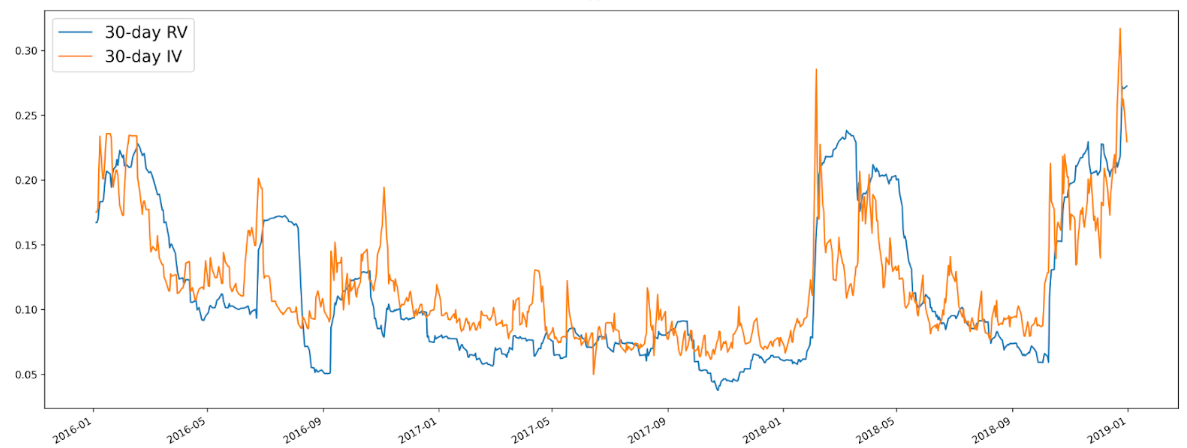
\includegraphics[width = \textwidth]{figures/iv_rv_spy.png}
    \caption{Trends of realized volatility and implied volatility of S\&P 500 options}
    \label{fig:iv_rv_spy}
\end{figure}

\section{Background}
\subsection{Options}

An option is a financial product that allows you to trade the future price of the market. When you purchase an option, you are buying the right to trade in the market at a fixed price on a specific date before the option expires, i.e., before the option expires. In this respect, options are similar to futures - but unlike futures, you are not obligated to trade if you don't want to. There are several options pricing models that use these parameters to determine the fair market value of an option. Of these, the Black-Scholes model \citep{Black1973May} is the most widely known. Other models are also commonly used, such as the binomial model and trinomial model.

%In many ways, options are just like any other investment—you need to understand what determines their price to use them effectively. 

The Black-Scholes model is one of the essential concepts in modern financial theory. This mathematical equation involves time and other risk factors to estimate the theoretical value of derivatives based on other investment instruments. This model follows geometric Brownian motion and therefore has constant drift and volatility. In the case of stock options, the model includes the strike price and expiration time of the option, the continuous value change of the stock, and the time value of money.

The Black-Scholes call option is calculated by multiplying the stock price by the cumulative standard normal probability distribution function and the exercise price by the cumulative standard average distribution net present value (NPV) minus the previously calculated resulting value.

\begin{center} 
$
\begin{matrix}
C=SN (d_1)-Ke^{-rt}N (d_2)
\end{matrix}
$
\end{center}

where:

\begin{center} 
$
\begin{matrix}
d_1 = {{ln^{S}_K+(r+{\sigma^{2}_v \over2} )t} \over \sigma_S \sqrt t}
\end{matrix}
$
\end{center}

and:

\begin{center} 
$
\begin{matrix}
d_2 = d_1-\sigma_S \sqrt t
\end{matrix}
$
\end{center}

and where:

\emph{C} = Call option price

\emph{S} = Current stock (or other underlying)

\emph{K} = Strike price 

\emph{r} = Risk-free interest rate 

\emph{t} = Time to maturity 

\emph{N} = A normal distribution



\subsection{Role of Volatility in Options Pricing}
The Black-Scholes equation requires five variables. These inputs are the price of the underlying asset, strike price of the option, time until expiration of the option, risk-free interest rate and volatility. With these variables, it is theoretically possible for options sellers to set rational prices for the options that they are selling. 

The values for all of the variables in this equation are known, except for volatility. The volatility in Black-Scholes equation is the future volatility of the underlying, and is hence unknown. In practice, the market determines the option prices through supply and demand on the exchange. From this price,
the volatility can be derived using a formula (such as the Black-Scholes formula). This is called \textbf{implied volatility}. Higher option prices lead to a higher estimate of implied volatility.


\subsection{Volatility Trading}

Since the option price is a function of the underlying stock volatility, we can create strategies to trade our fundamental beliefs about volatility. In order to trade based on volatility, we first need to \textbf{delta-hedge} our option positions. Delta-hedging ensures that our positions are neutral to changes in the underlying price. Only movement in volatility then affects the returns from our option positions. 

From the Black-Scholes equation for the call option, we can see that 
\begin{align*}
    \Delta &= \frac{d C}{d S} = N(d_1)\\
    \text{where}\\
    N(x) &= \frac{1}{\sqrt{2\pi}} \int_{\infty}^x \exp(-s^2/2) ds\\
    \text{and}\\
    d_1 &= {{ln^{S}_K+(r+{\sigma^{2}_v \over2} )t} \over \sigma_S \sqrt t}
\end{align*}
Here we keep the Black-Scholes model assumptions that the underlying price follows the Geometric Brownian motion
$$
dS = \mu S dt  + \sigma S dX
$$

Suppose there are two values of volatility - $\sigma_i$ is implied from the option market price and $\sigma_b$ is your belief about the underlying volatility. Suppose $\sigma_i \ge \sigma_b \implies C(\sigma_i) \ge C(\sigma_b)$ where $C$ is the price of a call option and is a function of the volatility.  

This means that the call option is overpriced in the market based on your beliefs about the underlying volatility. In order to profit in this situation, a strategy can be to sell the option contract in the market. When the price corrects to your beliefs about the volatility, you can buy back the cheaper option and make profit from the difference in prices. The PnL of this strategy is 
$$
C(\sigma_i) - C(\sigma_b)
$$

Suppose we sell the option at price $C^i$ today. We also delta-hedge by buying $\Delta^i S$ of the underlying. Tomorrow, the change in option price is $dC^i$ and the delta hedge is $\Delta^i dS$.  The total profit from today to tomorrow can be written as
\begin{align*}
    \text{Profit}_{t \rightarrow t+dt} &= -dC^i + \Delta^i dS + r(V^i - \Delta^iS) dt\\ 
    &= 1/2 (\sigma^2_i - \sigma^2_b) S^2 \Gamma^i dt
\end{align*}
Using Ito's lemma and derivation from \citep{ahmad2005free}.

We can add up the present value of these profits over all periods $t$ to get total profits of 
$$
\text{Profit} = \frac12 (\sigma^2_i - \sigma^2_b) \int_{t_0}^T \exp(-r(t-t_0))S^2\Gamma^idt
$$
which is \textbf{always positive} when the implied volatility is higher than the true realized volatility.

\subsection{Volatility Risk Premium}
The volatility risk premium is the amount by which the implied volatility of an options contract exceeds the future realized volatility of the underlying asset. In other words, it is the difference between the market's expectation of the volatility of the underlying asset and the realized volatility of the asset. The volatility risk premium arises because option buyers are willing to pay a premium for the right, but not the obligation, to buy or sell the underlying asset at a predetermined price (the strike price) on or before a certain date (the expiration date). This premium compensates the option seller for the potential volatility of the underlying asset.

For example, let's say that the expected future realized volatility of a stock is 30\%, but the implied volatility of an options contract on that stock is 35\%. In this case, the options contract would have a volatility risk premium of 5\%, which would be included in the price of the contract. Overall, the volatility risk premium is an important consideration for both buyers and sellers of options contracts, as it can have a significant impact on the potential profit or loss from the trade.

The existence of a steady volatility risk premium among equity index options is contested in literature. There is evidence of the existence of a consistent volatility risk premium in the Forex options markets as shown in \citep{dierckx_trading_2022, BhatRupeeDollar}. Similar premiums are shown to not exist in the equity index markets \citep{bondarenko2016analysis}, \citep{schulte2015performance} \citep{dapena2015index}. The reason is that there are many factors that affect the movement of equity prices and at any time, any of these factors could lead to a higher realized volatility. This eliminates any gains from premiums.

In our experiments, we validate the idea of whether there exists a volatility risk premium in index options that can be harvested to gain a profit over sufficiently long trading periods.

\subsection{Volatility Skew in Options}\label{volskew}
The implied volatility skew is the difference in implied volatility between options with different strike prices. Typically, options with lower strike prices have higher implied volatilities than those with higher strike prices, creating a \textit{skew} shape in the implied volatility curve. This skew is often referred to as the "smile" or a "smirk" because of its shape when plotted on a graph \citep{IVSmirk}. The implied volatility skew is important because it can have a significant impact on the value of options and option strategies.

Reverse skews occur when the implied volatility is higher on lower options strikes. It is most commonly seen in index options or other longer-term options. Put options with a lower strike price tend to have higher implied volatility than put options with a higher strike price. Lower-strike price (OTM) puts are often combined with long positions to provide downside protection. As a result, OTM puts tend to be in higher demand, leading to generally higher prices. Consequently, the implied volatility in OTM puts is higher, as compared to higher strike puts.

Clearly, the realized volatilities of these options with different implied volatility are the same since the underlying is the same. This provides an arbitrage opportunity, whereby selling an OTM put and buying an ATM put in the same underlying harvests the difference in implied volatility between these two contracts.


\subsection{Straddle Strategy}
The straddle options trading strategy is a neutral strategy in options trading that involves the simultaneous purchase of a call option and a put option on the same underlying asset $S$, with the same strike price $K$ and expiration date $T$. A trader can execute either a long or a short straddle strategy. The long straddle is designed to profit from significant moves in the price of the underlying asset, either upwards or downwards. On the other hand, a short straddle profits when volatility is low. 

The payoff from a long straddle is given by
\begin{align*}
    \text{payoff}(K, T) &= \text{put}(K,T) + \text{call}(K,T)\\
    &= \max(0, X-K) + \max(0, K - X)\\
    &= |X - K|
\end{align*}
where $X$ is the underlying price at any given time. 

The profit from a straddle is the payoff minus the cost of the straddle which is determined by the price of the put and call options on the market. As a straddle is just made up of a put and call option, its price can be determined using the Black-Scholes formula as

\begin{align*}
    \text{price} = S(N(d_1) - N(-d_1)) - Ke^{-rt}(N(d_2) - N(-d_2))
\end{align*}
This is the price we pay when we buy (long) a straddle. 


% If the price of the underlying asset increases significantly, the call option will increase in value, while the put option will decline in value. Conversely, if the price of the underlying asset decreases significantly, the put option will increase in value, while the call option will decline in value.

Straddle is a great strategy that can be used in a number of different market environments, from volatile markets, range-bound markets, to markets with low volatility. In volatile markets, the straddle strategy can be used to profit from significant moves in the price of the underlying asset, as the call and put options will both increase in value. If the trader anticipates high volatility, a long position on straddle gives an opportunity to profit whether the underlying increases or decreases.

In range-bound markets, the straddle strategy can be used to profit from the passage of time, as the time value of the options will decline as the expiration date approaches. In markets with low volatility, the short straddle strategy can be used to profit from a lack of movement in the price of the underlying asset, as the options will expire worthless. An ideal strategy in these markets will be to take a short position on the straddle, the payoff diagram for which is shown in Figure \ref{fig:short_straddle}. Consequently, the short straddle can be used in a way to harvest the volatility risk premium in options. 

Overall, the straddle options trading strategy is a versatile strategy that can be used to profit from a wide range of market environments and conditions. It is typically used by experienced options traders who have a good understanding of the risks and potential rewards of the strategy.

\begin{figure}[t]
\centering 
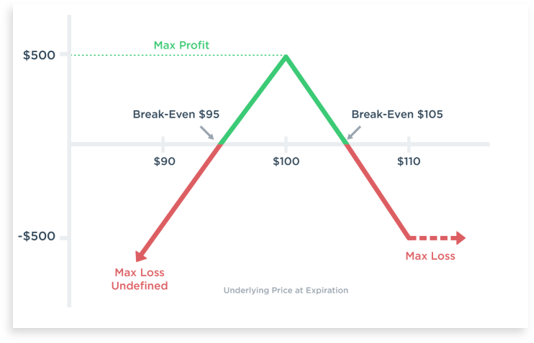
\includegraphics[width=0.7\textwidth]{Short Straddle PnL Plot.png} 
\caption{Short Straddle PnL Plot} 
\label{fig:short_straddle}
\end{figure}

\subsection{Random Forests Model}
A random forests model \citep{RFBreiman} is a type of machine learning model that uses an ensemble of decision trees to make predictions. A decision tree \citep{breiman1984classification} is a tree structure that splits the data into smaller and smaller subsets based on certain decision criteria. Each branch of the tree represents a possible decision, and each leaf node represents the outcome of that decision.

A decision tree makes branching decisions by using a set of rules that specify how to split the data at each node of the tree. To create these rules, the decision tree algorithm starts at the root node of the tree, which represents the entire dataset. It then evaluates each of the input features to determine which feature will result in the best split of the data. This is typically done by calculating a metric such as the Gini impurity or the information gain at each split and choosing the split that results in the lowest value of this metric. Once a split has been chosen, the algorithm creates two child nodes, one for each subset of the data. The process is then repeated at each child node, using the same procedure to evaluate the features and choose the best split. This continues until all of the leaf nodes of the tree are pure, or until some other stopping criterion is reached. Thus, the decision tree algorithm uses a set of rules to iteratively split the data into smaller and smaller subsets, until each leaf node contains a pure subset of the data. This allows the decision tree to make predictions about the class or decision of new input data based on the characteristics of the data at each leaf node. By using these rules to create a tree-like structure, the decision tree is able to represent complex relationships between the input features and the target variable in a clear and interpretable way.

In a random forests model, the decision trees are trained using a random subset of the data, and the predictions made by each individual tree are combined to make a final prediction. This process is repeated multiple times, with different subsets of the data and different combinations of decision trees, to create an ensemble of trees. The final prediction is made by taking the average of the predictions made by each of the individual trees in the ensemble.

Random forests models are typically used for classification tasks, where the goal is to predict a class label for a given input, or for regression tasks, where the goal is to predict a continuous value for a given input. One advantage of random forests models is that they can handle large and complex datasets, and they are relatively resistant to overfitting. Another benefit that makes them suitable for financial applications is their explainability -- it is possible to visualize their constituent decision trees and understand the decision-making criteria. They are also relatively easy to train and deploy, making them a popular choice for many machine learning tasks.

\section{Methods}
In this section, we describe our portfolio of market-neutral strategies. Our strategies aim to capture different volatility premiums in index options using options. Section \ref{straddle} defines a short straddle strategy that captures the volatility risk premium. Section \ref{strangle} defines a short strangle strategy that also captures the volatility risk premium but provides profit under greater price movement. In Section \ref{skew}, we propose a new strategy for capturing the volatility skew in put options - this strategy is termed as the \textit{Weighted Skew Arbitrage} strategy. Finally, in section \ref{rf}, we discuss a modification to our strategies by augmenting them with machine learning models.

\subsection{Short Straddle Strategy} \label{straddle}

A short straddle is a neutral strategy that involves
simultaneously selling a put and call in the same security, at the same strike price and the same expiration date. The idea is to harvest volatility risk premium in options. In this strategy, we sell one-month long straddles of notional value equal to the allocated portfolio value. For example, for a portfolio of \$1 million, we sell puts worth \$1M and calls worth \$1M in terms of notional value. Furthermore, dynamic delta hedging is performed twice a day, at 10AM and 2PM. The dynamic Delta hedging equation is as follows:

\begin{center} 
$
\begin{matrix}
Hedge(t) = -(\Delta{\text{call}} (t) + \Delta{\text{put}} (t)) * \textit{ContractUnit}
\end{matrix}
$
\end{center}
Here, $\Delta_{\text{put}}$ is negative, hence the terms mostly cancel out when the calls and puts are close to being at-the-money. As time proceeds and the underlying stock price moves, one of the contracts becomes OTM (which has a lower delta), while the other becomes ITM (which has a higher delta). Consequently, one side of the delta hedging equation dominates and dictates whether our underlying holding is net short or long. 

The contracts are held until the last trading day before expiration, upon which they are liquidated along with the underlying holdings. If the underlying's realized volatility remains under the implied volatility, we profit from the difference reflected in the final price of the options, minus the cost of rebalancing the delta hedge.

\subsection{Weekly Short Strangle Strategy} \label{strangle}
Inspired by Dierckx et al. \cite{dierckx_trading_2022}, we implemented a strategy selling short-term strangles every day. A new 5-day SPY strangle is bought at 10AM Central Time, with a notional value equal to 1/\nth{5} of the total portfolio value. The entire portfolio is delta-hedged with SPY twice a day, once at 10AM and once at 2PM. The strikes are chosen to be as close as possible to the spot while satisfying the constraints:
\begin{align*}
    K_{Put} \leq SPY_t - \textrm{strangle\_size} \cdot SPY_t \cdot \sigma_{60}, \quad K_{Call} \geq SPY_t + \textrm{strangle\_size} \cdot SPY_t \cdot \sigma_{60},
\end{align*}
where $\sigma_{60}$ is the 60-day realized volatility of SPY. That is, the width of the strikes is scaled with the price times the volatility of SPY; this allows for risk to be mitigated in volatile periods while still capturing a healthy-sized premium during normal market conditions. For example, for $strangle\_size = 0.1$, 
\begin{align*}
    K \approx SPY_t \pm \$2\ \textrm{  in 2017} \quad \textrm{and} \quad K \approx SPY_t \pm \$10\ \textrm{ in 2022}.
\end{align*} We compare the strategies for various values of \textit{strangle\_size} $\in [0,0.05,0.1]$ in Table \ref{ResultsStrangle}. We found in backtesting that generally selling strangles with wider strikes results in a higher Sharpe ratio for this strategy, while reducing returns in some cases.

There are some interesting consequences of delta-hedging multiple strangles per day. To hold strangles $\{(call_i, put_i) \times q_i \}$, the required amount of underlying holdings is 
\begin{align}
    \text{Stock Holdings Quantity} = \sum_i q_i (\Delta_{put_i} + \Delta_{call_i}) \cdot 100.
\end{align}
Therefore each term can have potentially different signs, leading to a cancellation of deltas.  Hence on average, the stock uses less margin, compared with holding a single type of strangle, where at expiry the combined delta is always $+1$, $-1$, or $0$. In this case we potentially have to long or short the entire notional value near expiry.

Furthermore, the returns on a delta-hedged strangle tend to be lower but more consistent compared to straddles. Recall that the PnL for delta-hedged short options is path-dependent, and can be calculated based on the idealized formula
\begin{align}
    PnL = \frac12 \int S_t \Gamma_t (\sigma_i^2 - \sigma_r^2).
\end{align}
From Figure \ref{fig:gamma_plot}, the $\Gamma$ of a straddle is strongly peaked at the strike, whereas $\Gamma$ is more spread out between the strikes for a strangle. Thus straddles capture VRP if $S_t$ remains close to the strike, and does not have much PnL if $S_t$ drifts far away. In contrast, $\Gamma$ remains at a more consistent albiet lower level throughout the strike range, hence we can capture VRP even when the stock price drifts from its initial value, as long as the spot remains in between the strikes.

\begin{figure}[t]
\centering 
  \centering
  \subfloat[Straddle.]{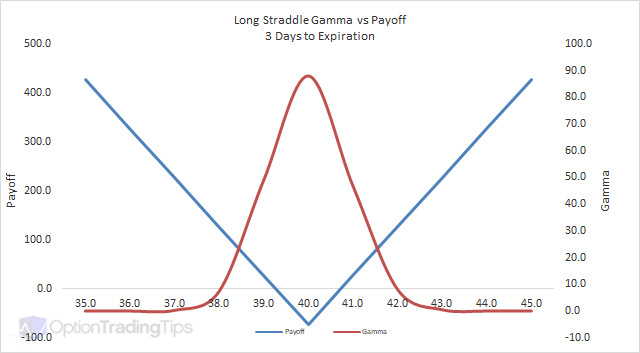
\includegraphics[width=0.5\textwidth]{straddlegamma.png}\label{fig:f1}}
  \hfill
  \subfloat[Strangle.]{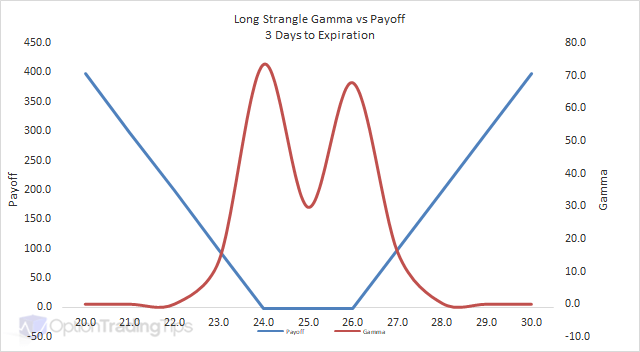
\includegraphics[width=0.5\textwidth]{stranglegamma.png}\label{fig:f2}}
  \caption{$\Gamma$ comparison}
\label{fig:gamma_plot}
\end{figure}

\subsection{Weighted Skew Arbitrage Strategy}\label{skew}
In this subsection, we propose a strategy for harvesting the implied volatility skew in put options, as detailed in section \ref{volskew}. The strategy is as follows. Sell OTM put contracts at strike $K_2$ and buy ATM put contracts at strike $K_1$ (where $K_1 > K_2$) in the ratio of $\lambda: 1$, where $\lambda$ is a parameter we define. In other words, for each ATM put purchased, we sell $\lambda$ OTM puts. The portfolio is delta-hedged daily, by maintaining a holding of $\Delta * S$, where $S$ is the number of stocks represented by the option and $\Delta = \Delta_{\text{ATM}} - \lambda\Delta_{\text{OTM}}$. Now, we derive the returns from this strategy.

First, consider a delta-hedged long strategy for an option with strike $K_i$. We define the following variables: $S$ is the units of the underlying represented by an option; $\sigma_{r}$ is the realized volatility; $\sigma_i$ is the implied volatility in contract $i$; $\Gamma_t$ is the option Greek Gamma at time $t$. Based on the work of \citep{ahmad2005free}, the returns for this strategy, $d V_i$ can be calculated as: 
\begin{align}\label{skewEqn}
    d V_i = \frac12 S^2 \Gamma_t (\sigma_r^2 - \sigma_i^2) d t
\end{align}

The weighted skew arbitrage strategy can be decomposed into two separate delta-hedged strategies - one with a long ATM put option, and the other with $\lambda$ options of the OTM puts. Using \ref{skewEqn} we can obtain the change in the portfolio value of our strategy $V$ as follows:
\begin{align*}
    d V = \frac12 S^2 \Gamma_1 (\sigma_r^2 - \sigma_1^2) d t - \lambda \frac12 S^2 \Gamma_2 (\sigma_r^2 - \sigma_2^2) d t + P(K_2) d \lambda
\end{align*}
Here, the indices $i=1$ correspond to the long ATM put, and $i=2$ corresponds to the short OTM puts. $\Gamma_1, \Gamma_2$ are used in place of $\Gamma_t$ for the respective options. The extra term $P(K_2) d \lambda$ reflects the change in lambda itself, which could change the number of OTM options we short. 

Now, we propose the value of $\lambda = \frac{\Gamma_1}{\Gamma_2}$. Using this, the above equation can be simplified as:
\begin{align*}
    d V &= \frac12 S^2 \Gamma_1 (\sigma_r^2 - \sigma_1^2) d t - \frac12 S^2 \Gamma_1 (\sigma_r^2 - \sigma_2^2) d t + P(K_2) d \lambda \\
    &= \frac12 S^2 \Gamma_1 (\sigma_2^2 - \sigma_1^2) d t + P(K_2) d \lambda \\
\end{align*}
Now, because of the implied volatility skew generally found in put options, $\sigma_2 > \sigma_1$. Hence, this strategy is profitable in expectation, because the change in portfolio value $d V$ is positive.

A crucial aspect of implementing this strategy is determining which values of $\Gamma$ to use. Generally, $\Gamma$ changes with time and can hold many different values during an option's lifetime. There are two approaches to this. The first approach is to dynamically balance $\lambda = \frac{\Gamma_1}{\Gamma_2}$. This is similar to dynamic delta hedging and ensures that we always hold the appropriate number of options (long and short) to adjust for any underlying price changes. However, a limitation of this approach is that this requires frequently buying and selling options. In comparison to stocks, option prices are much more volatile and rapidly buying or selling large amounts of options can cause much larger losses than dynamic delta hedging as option prices can shoot up or down over time. The second approach is to determine a reasonable $\lambda$ value based on recent historical data. To determine an appropriate static value for $\lambda$, we could consider the following. 

\begin{align}\label{lambdaEqn}
    \lambda = E_S \left[ \frac{\int_0^T \Gamma_2 d t}{\int_0^T \Gamma_1 d t}\right]
\end{align}
The expectation is taken over all stock paths of $S$ from time 0 to $T$. For this value of $\lambda$, we get an expected PnL of:
$$E_S[PnL(0,T)] = \frac12 (\sigma_2^2 - \sigma_1^2) E_S\left[\int_0^T \Gamma_1 S^2 d t\right]$$
This is a positive value, implying a profitable payoff. Unfortunately, computing this value of lambda is intractable because it is very hard to determine all possible stock paths of $S$. However, this approach provides a hint for computing a suitable $\lambda$. We consider historical data over the past 90 days and compute a mean of $\lambda = \frac{\Gamma_1}{\Gamma_2}$ values over this data. This provides an estimation of $\lambda$ in equation \ref{lambdaEqn} over reasonable stock paths in recent history. This is the approach we implemented in our strategy. Results and discussion of the strategy will be included in forthcoming sections.
 
%Skew arbitrage is a type of statistical arbitrage implemented by trading a delta and volatility-neutral portfolio. The objective is to take advantage of differences between the implied skew and a forecast of the future realized skew of the option's underlier.

%Skew "arbitrage" is a pretty broad term. When you are trading the skew, there are 3 principal risks:

% \begin{itemize}
% \item The actual change in the slope of the skew in the implied space. e.g., if you are trading 95\% strike against a 105\% strike and your underlying stays in place, all of your instantaneous P&L would be due to the changes in the implied vol at each strike time, the vega per leg.
% \item Realization of volatility across the striking space. If the underlying drifts to one of the strikes, what would be the volatility realized along the way, and how it relates to the original difference in vols that you locked.
% \item The implied volatility across the realized strike space. If the underlying goes to the vicinity of one of the two strikes, what would be the implied volatility you have to buy back or sell.
% \end{itemize}

\subsection{Machine Learning Augmented Trading} \label{rf}
Machine learning is a valuable tool in quantitative finance. We utilize ML as a secondary signal to make trading decisions in our strategy. We propose a decision model to trade based on the predicted Sharpe ratio. 

A recent paper by \citet{dierckx_trading_2022} proposed a random forests model to predict the closing Sharpe ratio of one-week delta-hedged straddles. The paper showed that this ML-augmented strategy outperformed the naive strategy for EUR-USD straddles.

To replicate this strategy for SPY options, due to higher volatility causing losses for straddles, we augment our strangle strategy $\textit{strangle\_size}= 0.1$. As noted prior, we found that the weekly strangle strategy performed with a higher Sharpe ratio than using straddles on in-sample data.

\subsubsection*{Description of strategies}

We implement a similar approach for predicting whether a trade in our strategy will be profitable. Using sklearn's RandomForestClassifier, a random forest model is trained to predict the closing Sharpe ratio of short one-week delta-hedged strangles. As percent return of a single trade is not well-defined, the formula for the Sharpe ratio for a given delta-hedge traded in our strategies is given by:

\begin{center} 
$
\begin{matrix}
Sharpe \,  Ratio^* = {E[P \& L] \over \sigma_{[P\&L]} }.
\end{matrix}
$
\end{center}

 On any given trading day, we attempt to predict the Sharpe ratio of starting a delta-hedged straddle opened at time $t$ and expiring $t+ 5$ trading days in the future. For a trade opened at time $t$, define the objective functions $y_i(t)$:
$$ y_1(t)=\left\{
\begin{aligned}
1,  & \ \text{ if Sharpe ratio(t+5) < -0.25} \\ \\
0,  &\ \text{ otherwise}
\end{aligned}
\right. , \quad  y_2(t)=\left\{
\begin{aligned}
1,  & \ \text{ if Sharpe ratio(t+5) > 0.3} \\ \\
0,  &\ \text{ otherwise}
\end{aligned}
\right. .
$$

In other words, $y_1$ is the bad day indicator, and $y_2$ indicates a good day to trade. We train random forest classifiers on both, with 2 years of historical data, while periodically retraining on the most recent 2 years every 4 months. Let $P(y_i)$ be the random forest probability prediction of $y_i$. With these 2 indicators we develop the following two strategies:
\begin{enumerate}
    \item $S_1$: \textit{Bad day prevention}. Place trade when $P(y_1) < c_1$, otherwise do not trade. Initialize $c_1 = 0.16$. Dynamically adjust $c_1$ to keep the algorithm trading 70\% - 85\% of the time.
    \item $S_2$: \textit{Bad day prevention with boost}. Same bad day prevention criterion as $S_1$. If $P(y_2) > 0.5$ sell double the usual quantity of strangles, if available margin is more than 25\% of the total portfolio value.
\end{enumerate}

\subsubsection*{Dynamic Threshold Adjustment for $y_1$}

In \cite{dierckx_trading_2022}, the RF outputs were converted into true via. the better RF models reduced the trading frequency by a calibration scheme based on training data; however trying this method ended up making the probabilities even more inconsistent for our data. In their paper, the trading frequency was reduced fair amount, so the threshold for $y_1$ is dynamically tuned to produce a target trading frequency of 70 \% - 90 \% in the last 22 days in lieu of having have a target probability. The daily update algorithm for $c_1$ is as follows:

Initialize $c_1 = 0.16$. Let $T(t) = 1$ if we traded on day $t$, and $T(t) = 0$ otherwise. For each day, if $EMA_{22}(T)(t) > 0.85$, reduce $c_1$ by 0.001, and if $EMA_{22}(T)(t) < 0.7$, increase $c_1$ by 0.001. A lower $c_1$ is more restrictive on trading, whereas a lower $c_1$ is more permissive. This keeps the algorithm trading at a relatively consistent rate. A threshold adjustment scheme is necessary because the output of a RF classifier (other than the value 0.5) does not represent a true probability as it is simply a vote of the random decision trees in the forest. We found empirically that a fixed threshold leads to the $y_1$ model being too restrictive during some years, while other years it would be too lenient.

\subsubsection*{Feature Design}
Our model uses the following 10 features:
\begin{multicols}{2}
\begin{itemize}
  \setlength\itemsep{0em}
	\item End-of-day return for the underlying
	\item 30-day implied volatility
 	\item 30-day rolling realized volatility
    \item 5-day implied volatility
    \item 5-day rolling realized volatility
 	\item 30-day-IV rank (lookback 100 trading days)
    \item 5-day-IV rank (lookback 22 trading days)
    \item Difference between implied and rolling realized volatility (both timeframes)
    \item Sharpe ratio of trade started on $t-5$ trading days
	\item Hit rate – (lookback $[t- 5 - 22, t - 5]$ trading days).
\end{itemize}
\end{multicols}
In addition, we include the day of week and an extra $10 \times 3$ features based on difference from previous day, difference from 30-day EMA, and rolling 30-day standard deviation to capture temporal information.

\subsubsection*{Software Development}
Due to QuantConnect's lack of implementation of a Short Straddle Option strategy, a class called DeltaHedgedStraddleTracker was written to keep track of the individual PnL of multiple straddles at once including its delta, and to handle the Sharpe ratio calculation upon expiry. An algorithm was written to virtually sell a straddle every day and save the data from 2012-2022. Another script was also written to harvest historical IV of ATM put and calls and RV data from 2012-2022 and save to file. We aggregated this data in the QC research environment and saved it onto 2 files: features and Sharpe ratios from 2012-2022.

For our ML augmented algorithm, we simply pulled data from these files to train a random forest, making sure to not have lookforward bias. Therefore the ML portion of our project only works for backtesting. In order to do live trading with this, future work involves writing a full algorithm that is able to pull all the relevant data live, as well as save the Sharpe ratio of trades, generating training data to train on periodically.

\subsubsection*{Parameter selection}

The sklearn random forest parameters are as follows:
\begin{multicols}{3}
\begin{itemize}
  \setlength\itemsep{0em}
    \item n\_estimators = 300
    \item max\_depth = 6
    \item min\_samples\_split = 2 
    \item min\_samples\_leaf = 50
    \item random\_state = 42
    \item max\_features = 0.25.
\end{itemize}
\end{multicols}
We found that reducing the max\_features and increasing the min\_samples\_leaf resulted in less overfitting.

\subsubsection*{Cross-Validation and Model evaluation} We evaluated our models by walking forward through test data from the in-sample period in 3 month increments, and training on the most recent 3 months. Based on accuracy metric, we encountered issues due to overfitting, as the models had much worse accuracy on test data than training data. However, for the purposes of trading, we did not need the RF to identify all or even most of the $y_i = 1$'s, just that when it does register that $y_i = 1$, it does better than random. In other words, we can afford to not care so much about false negatives, as long as the model is better than random when it does does send a trading signal.

To evaluate our indicators more thoroughly, we looked at the average partial AUC-ROC, an overall measure for how much a classifier is at predicting true positives for a given acceptable level of false positives. 

The ROC curve, or receiver operating characteristic curve, plots the true positive rate against the false positive rate of a binary classifier under various thresholds. See Figure \ref{fig:ROC}. A `useless' classifier will predict positive for the same proportion of actual positives as it does for actual negatives. Therefore a ROC curve above the diagonal line indicates that the classifier is actually doing better than chance. AUC-ROC is the area underneath this curve, and `partial' refers to only examining the region of the curve where false positives are low; in our case we set the max false positive rate to 0.4. The score is normalized so that 0.5 represents a dummy classifier, any score > 0.5 beats the dummy. Our two strategies are designed to perform similar to baseline even if the classifier is as good as random. In light of this, partial AUC-ROC is a suitable evaluation metric for our problem since we want to allow the indicator to be fairly weak at finding the exceptional days, but make sure it is better at selecting the exceptional days over it is at selecting the non-exceptional days.

The average AUC-ROC score over the period 1/1/2017 - 1/1/2021 was $(0.61, \sigma = 0.11)$ for $y_1$ and $(0.53, \sigma = 0.04)$ for $y_2$, which indicates that classifier did learn \textit{some} information about the Sharpe ratio. For example, the ROC curve for $y_2$ in early 2020 in Figure \ref{fig:ROC} is exceptionally good. But for other 4-month spans the curve is below the diagonal, indicating that the model is predicting false positives more often than random! It is somewhat surprising then that $S_2$ increased the Sharpe ratio over $S_1$ for all testing periods. As we will see, both ML-augmented strategies did fairly well in terms of Sharpe ratio.
 
\begin{figure}[h]
    \centering
    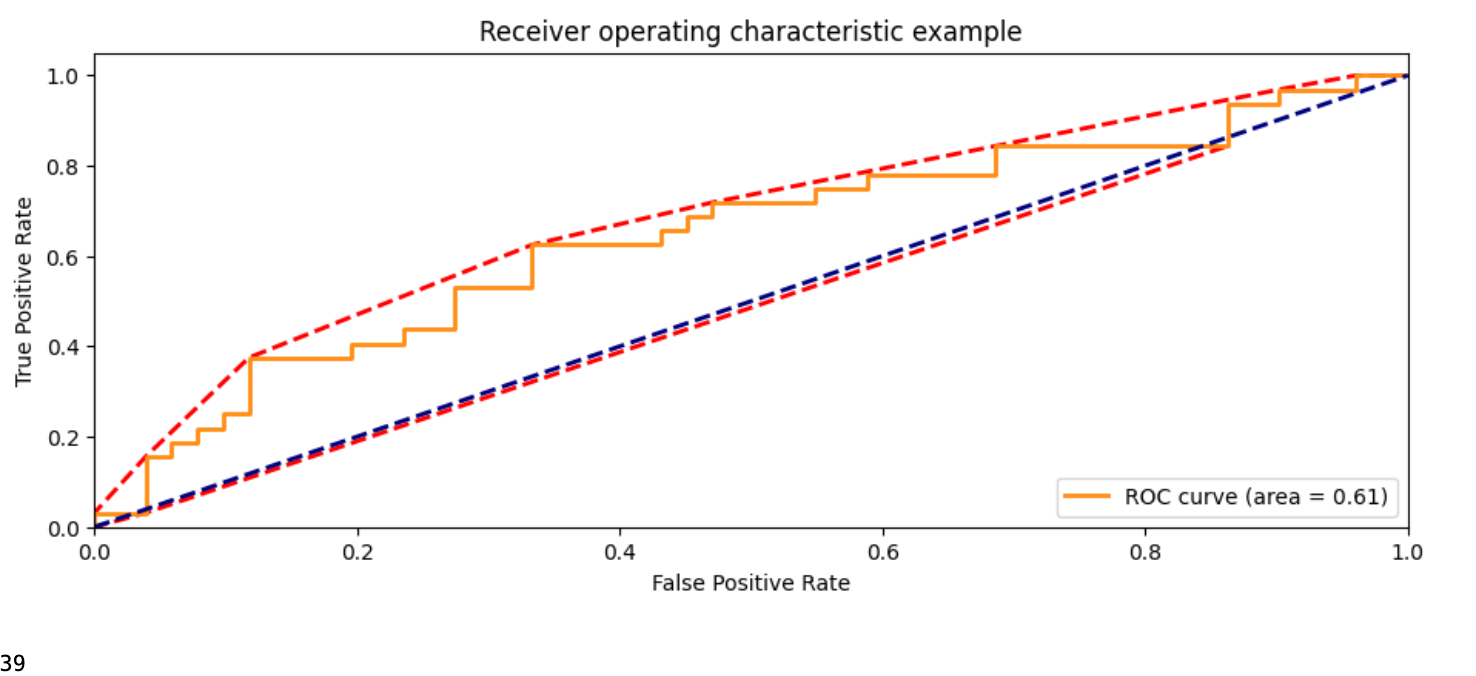
\includegraphics[width=0.7\textwidth]{ROCcurveEarly2020.png}
    \caption{ROC curve of $y_2$ during first four months of 2020}
    \label{fig:ROC}
\end{figure}


\section{Implementation}
\subsection{Selection of Underlying Security}
The first step in implementing our strategy ideas is to pick an underlying for the options. Options are available for a wide variety of securities. For our strategies, a few constraints are crucial. We require an underlying whose options have high liquidity, to allow for easily closing positions at any time during the trade. Furthermore, the underlying should \textit{generally} have low volatility. For high volatility instruments there may exist a volatility risk premium, but it is difficult to predict the consistency of this premium. Thus, lower volatility securities are preferred as the underlying. Finally, the extent of peer-reviewed research on similar volatility trading strategies is also a factor for selecting the class of underlying assets.

Table \ref{underlying-table} compares different classes of options based on the underlying. Individual equities were not considered for our stratagies, mainly due to relatively lower derivative liquidity, and higher volatility. Options based on indexes, forex and futures are generally best suited for our strategy, and also more widely studied in the literature. 

\begin{table}[h]
\centering
\begin{tabular}{ccc}
\toprule
\textbf{Index Options} & \textbf{Forex Options} & \textbf{Futures Options} \\\midrule
High liquidity & High liquidity & Liquidity may be lower \\
Low volatility & Low volatility & Low volatility \\
{\makecell{Some studies on VRP \\ in literature}} & {\makecell{Many studies on stable VRP  \\  in literature }} & {\makecell{Few studies on VRP  \\  in literature}} \\\toprule
\end{tabular}
\caption{Characteristics of different options}
\label{underlying-table}
\end{table}

The best candidates for testing our strategy were index and forex options - based on liquidity and volatility requirements, as well as the extent of research. We decided to go with Index options for the following reasons. Our algorithmic trading platform, QuantConnect, provides high-quality cleaned/parsed data for index options. Index options have high liquidity and availability of many short-maturity options. Trading and brokerage fees are more economical in index options.

Our experiments and backtests were performed trading on \textbf{SPY options}. This is the ticker for the index that tracks the Standard \& Poor's top 500 companies by market capitalization (S\&P 500).


\subsection{Risk Management}
Our strategies attempt to capture the volatility premium in options by waiting out our positions until the options expiration date. Because we are selling options in our strategies, the most significant risk factor is the potential drastic increase in short-term volatility, which could potentially wipe out the portfolio if proper risk management practices are not set. Even with sophisticated machine learning algorithms that achieve high prediction accuracy, one false prediction coupled with weak risk management can obviously mean the end of a portfolio. This section explores the four main risk management strategies we implemented.
% \begin{itemize}
% 	\item Stop-loss
% 	\item VIX-based
%         \item Delta-based
%         \item Kelly's Criterion
% \end{itemize}
\subsubsection{Stop-loss}
The first risk-management approach was a stop-loss based on percentage $\alpha$ of current total portfolio value. We tuned the parameter of the strategy (stop-loss threshold) by running backtests with different stop-loss percentage values. Different values of $\alpha$ resulted in drastically different returns for the same strategy. We found that higher $\alpha$ leads to higher drawdowns which severely impacted the overall return of the portfolio for the period. We noticed that often when there are sharp movements in price during the course of a trade, only a few large price movements can cause losses that are hard to recover from. This is because our strategy makes money when volatility is low, so even a few large price movements can make the recovery hard when options expire. As a result, it is better to close our positions when we experience a somewhat large shock to our holdings.

We tested the following stop-loss threshold $\alpha$ values: 1\%, 2\%, 5\%, 10\%, 20\% of total portfolio value. It was found that it is generally beneficial to exit out of trades that lose more than 2\% of the capital invested instead of waiting until the expiration date in hopes of trade turning a profit. Because our strategy sells options, the value at risk (VaR) is very high upon option exercise. Therefore, it makes sense that conservative stop-loss thresholds produce the best results for controlling the risk. For $\alpha \geq 20\%$, the stop-loss condition is never hit. Thus, for best performance, a \textbf{stop-loss threshold of $2\%$ was used}.

\subsubsection{VIX-based}
VIX, typicall known as the "fear index," is the ticker symbol for the CBOE Volatility Index, which reflects the expectation of volatility based on S\&P 500 index options. Historically speaking, VIX values above 30 indicate a greater level of fear and uncertainty in the market whereas values below 30 indicate stability and investor confidence. 

Since all of our strategies short volatility, VIX seemed like a good source of insight for future volatility movement in the market. The risk management strategy is to exit out of our trades when VIX increases substantially in anticipation of the implied volatility eventually catching up with VIX. An increase in implied volatility would mean an increase in the options price, which would negatively affect the portfolio return. 

VXX (weighted average of 60-day volatilities) and VIX (weighted average of 30-day volatilities) values were compared. If VIX is higher than VXX, it can indicate that the market is anticipating a short-term increase in volatility and vice versa. Based on these signals, we could exit out of trades early in anticipation that volatility will continue to increase in the short term. However, after tuning the hyperparameters and running several backtests with the exit strategy based on VIX/VXX, we found that the strategy based on VIX underperforms. While sound in theory, there are three main problems with the strategy:
\begin{itemize}
	\item VIX values and IV values are not directly comparable: VIX was usually around 20 whereas the individual implied volatilities for the index options were around 40
	\item Using VIX/VXX ultimately means we have to be able to predict future volatility
        \item Stop-loss is always called before VIX-based conditions are met
\end{itemize}

First problem is that volatility represented by VIX cannot directly be compared to the implied volatility of the index options. For the time period tested, VIX was usually around 20 whereas the individual implied volatilities for the index options were around 40. Therefore, direct comparison between the two quantities was not possible, which made a risk management strategy based on directly comparing the two values somewhat arbitrary because we would need to multiply some factor to VIX in order to compare the two.

The second problem is that even when we observe a divergence between VIX and VXX, we have to decide whether volatility has permanently shifted and thus IV would catch up to VIX or whether the shift is temporary and that VIX would come back down to the original, historical level. Comparing VIX to VXX is equivalent to comparing different SMA's with each other. Just because a 30-day SMA crossed the 60-day SMA from the bottom, it does not always mean that the momentum has shifted. These crossover signals could serve as meaningful indicators but could also be false signals. Therefore, it implies that our trading strategies need to have other measures to determine whether the short-term shift in VIX is permanent or not. Doing so is equivalent to trying to profit from directly trading the volatility and diverges from our main strategy of capturing the volatility premium because it introduces another source of uncertainty.

The third problem is that in the event that the VIX condition does get triggered, we found that stop-loss is almost always triggered first because our stop-loss thresholds are conservatively set (at 2\% based on hyperparameter tuning). Because VIX is a reflection of the expectation of the volatility for S\&P index options, an increase in VIX usually leads to an immediate increase in IV, which readily increases the loss for our strategy. The strategy implemented with stop-loss is always triggered as a result. Therefore, we can only know from hindsight that VIX would have predicted an increase in IV for that specific trade but we were not able to capitalize on VIX because stop-loss was enough to prevent our losses.

\subsubsection{Delta-based}
One of the main risks with option-selling strategies is the gap risk. Gap risk is the risk from sudden drastic movements in the underlying's price. Delta hedging ensures that our positions are protected from movements in the underlying's price. However, the trader must continuously rebalance to account for changes in delta. Dynamically balancing the delta causes losses for the trader. This is because when the underlying's price increases, the overall delta increases, which requires buying more of the underlying to rebalance (and the opposite when price falls).  Effectively, the trader must buy high and sell low in the underlying in order to dynamically hedge their position's delta. 

If the underlying's price moves gradually, the losses accrued by delta hedging are low -- provided the trader diligently performs the (loss-making) delta hedge trades. However, if there is a sudden jump in the price of the underlying, the trader is exposed to gap risk as they may lose a large amount of money attempting to cover the change in delta due to this jump. Having large swings in the option delta causes immediate losses when adjusting our delta hedge, and also leads to higher option prices due to large volatility. These losses are hard to recover from, and as such, it may be better to liquidate our positions and cap the loss.

We propose monitoring change in delta as a risk-management approach. We utilized an approach that closes our positions if there is a sharp change in our net delta. Define $\delta{\Delta}$ as the change in delta for an option in a one-time step. For the straddle/strangle strategies, our portfolio change in delta is: $$\delta{\Delta} = \delta(\Delta_{put} - \Delta_{call})$$
If $\delta{\Delta} > \kappa$, then we liquidate our positions and do not perform the delta hedge. We implemented this strategy with $\kappa \in \{0.5, 0.75, 1\}$; for $\kappa=0.75$ we observed the best performance. This strategy is able to prevent many large loss-making trades, where it is better to close our positions after a large jump in price. This risk management approach performed better than VIX-based risk management because it predicts adverse price movements better than VIX (which is usually late in predicting swings in implied volatility). Though, the overall performance was equivalent, or occasionally slightly worse to stop-loss risk management. This is because sometimes delta-based risk management closed out some trades that eventually ended up being less destructive. 

\subsubsection{Kelly's Criterion}
Kelly's criterion is a formula that determines the optimal theoretical size for a trade given that expected returns are clearly known. As can be seen from the variables below, the expected return for profit and loss must be known in order for Kelly's criterion to be relevant to trading. Unlike most momentum-based strategies whose expected profit for individual trades is relatively arbitrary and varies a lot, the expected returns for our strategies are relatively predictable since the volatility premium we are trying to capture is relatively clear when we enter the trades and since the risk management strategies above give us a clear bound for our losses. If we can accurately predict the probability of loss/profit, since the expected profit is clear at the beginning of the trade, we could calculate $a$ which would serve as the optimal stop-loss threshold for that trade. Once $a$ is determined, we could know the optimal fraction of the assets to allocate to the trade. As the formula suggests, the higher the $a$, the lower $f^*$, which makes intuitive sense since a trade with a potentially higher expected loss is more likely to wipe out the portfolio. Therefore, we would allocate less capital to that trade, and vice versa.
$$f^* = \frac{p}{a} - \frac{q}{b}$$
\begin{align*}
    f^*&: \text{fraction of the assets to allocate to the trade}\\
p&: \text{probability of profit}\\
q&: \text{probability of loss}\\
a&: \text{expected loss}\\
b&: \text{expected profit}
\end{align*}


\subsection{Portfolio Diversification}
Portfolio diversification is one of the key aspects of constructing a portfolio. A portfolio that is well-diversified would have similar expected returns with lower Value at Risk (VaR), lower volatility, and a higher Sharpe ratio. We implemented a diversified version of our short straddle strategy over a portfolio of 3 index options. First, we considered the group \{\texttt{SPY}, \texttt{QQQ}, \texttt{XLF}\}. \texttt{SPY} is the ETF for the S\&P 500 index; \texttt{QQQ} is an index that tracks the 100 largest non-financial companies listed on the Nasdaq; \texttt{XLF} is an index that tracks the top financial companies in the S\&P500.

The above diversification strategy actually performed worse compared to the baseline strategy involving only SPY options. This diversified strategy obtains a return of 9.19\% and a Sharpe ratio of 0.583 for the in-sample period 2017-2021. Similar (worse) results are found in other out-of-sample periods as well. The reason for worse performance could be that there is a moderate correlation among the three indices; all three indices share a number of the same underlying assets. Another explanation is that tech stocks have been volatile at various points in time, especially since the COVID-19 pandemic and could have a negative effect on the portfolio.

Next, we considered three index options that are less correlated: \{\texttt{SPY, XLV, IWM}\}. \texttt{XLV} is an index that tracks major health sector corporations; \texttt{IWM} is an index composed of 2000 small-capitalization US equities. We found that when the portfolio is constructed with less correlated index options, the performance of the strategy improved. Table \ref{ResultsDiversification} demonstrates the results for the second uncorrelated diversification strategy. Diversification could increase the overall return of the portfolio when constructed with less correlated index options. However, the diversification strategy has a larger drawdown than any of the individual strategies. A better selection of uncorrelated index options could help alleviate the drawdowns and improve the returns. More research on selecting uncorrelated underlying assets could be considered for future work.  

\begin{table}[h]
\begin{center}
\begin{tabular}{@{}lcccc @{}}
\toprule
\textbf{Portfolio} & \textbf{Period}      & \textbf{Returns} & \textbf{Sharpe Ratio} & \textbf{Drawdown (duration)} \\ \midrule
SPY & 1/1/2017 – 1/1/2021  & 28.62\%  & 1.26 & 4.7\% (<1 month)\\
XLV & 1/1/2017 – 1/1/2021 &  7.87\% & 0.766 & 1,9\% (<1 month) \\
IWM & 1/1/2017 – 1/1/2021  & 11.28\%   & 0.853 &  1.7\% (< 1 month)\\
SPY, XLV, IWM &  1/1/2017 – 1/1/2021  &  26.59\% & 0.897 & 8.9\% (2.5 months) \\
SPY, XLV, IWM &  1/1/2010 – 1/1/2011  &  3.37\% & 1.992 & 1.3\% (2 months)\\
SPY, XLV, IWM &  1/1/2016 – 1/1/2017 &  1.57\% & 0.311 & 3.2\% (2 months)\\
SPY, XLV, IWM &  1/1/2022 – 11/1/2022  & -5.98\% & -0.995 & 6.2\% (3 months)
\\\midrule
\end{tabular}
\caption{Results for Portfolio Diversification}
\label{ResultsDiversification}
\end{center}
\end{table}


\subsection{Backtesting Approach}
For our backtesting, we used the QuantConnect platform. The following were important components of our backtesting strategies across various periods 
\begin{enumerate}
    \item \textbf{Including fees} - We used the QuantConnect \texttt{BrokerageModelSecurityInitialize} to initialize our brokerage model according to Interactive Brokers rates. This allowed us to have a good understanding of the fees incurred by our trades, and gave us a more accurate picture before running our strategy on live data
    \item \textbf{Parameterized and modular code} - During the development stages, we placed an emphasis on having modular and parameterized code, so that we can run several backtests quickly after changing the parameters. This allowed us to experiment with many different strategies with small tweaks and identify the parameters which worked the best. Some of the parameters we experimented with were -
    \begin{enumerate}
        \item \textit{Sharpe ratio thresholds} to help train the Sharpe ratio Random Forest classification model
        \item \textit{Stop loss thresholds} : After experimenting with several different values, we finally used 2\% threshold for our model
        \item \textit{Leverage} : to test the margin requirements of our strategy and experimenting with leverage to get more returns
        \item \textit{Strangle size} : varied the strangle size to see which strangles could best balance high returns and most volatility
    \end{enumerate}
    \item \textbf{In-sample period} - Our models were trained on the in-sample period of 1/1/2017 to 1/1/2021. Almost all of our models performed well in this period, which is important because this period included the covid months with some of the highest volatility in the recent years. In general, the recovery of the market after the covid period was stable and increasing, which led to good returns in our strategy
    \item \textbf{Out-of-sample period} - We tested our models on 3 out-of-sample periods.
    \begin{enumerate}
        \item 1/1/2022-11/1/2022 (Key: OS-A)
        \item 1/1/2016-1/1/2017 (Key: OS-B)
        \item 1/1/2010-1/1/2011 (Key: OS-C)
    \end{enumerate}
\end{enumerate}

\subsection{Evaluation Metrics} \label{evalmetrics}
We consider the following evaluation metrics for our strategies
\begin{enumerate}
    \item \textbf{Returns:} This reflects the gains (or losses) realized by our portfolio in the trading period
    \item \textbf{Sharpe ratio:} In the simplest form, Sharpe ratio quantifies the risk-adjusted returns to a portfolio \footnote{https://www.investopedia.com/terms/s/sharperatio.asp}. It's formula is 
    $$
    SR = \frac{R_p- R_f}{\sigma_p}
    $$where $R_p$ is the portfolio return, $R_f$ is the risk-free returns and $\sigma_p$ reflects the risk in the portfolio. The intuition behind Sharpe Ratio as a metric over returns is that at time, higher returns may indicate higher risks rather than better strategy.
    \item \textbf{Drawdown:} Drawdown refers to how much the portfolio is down from the peak before it recovers back to the peak. Drawdown management is important because if unrestricted, the entire portfolio equity could be lost in a huge drawdown event. Also, a high drawdown requires a much higher return to get back to previous levels. Drawdowns are represented as a percentage between peak and trough. 
\end{enumerate}

\section{Results}
In this section, we provide the results for our strategies. We note that there are several different settings and parameters that affect the strategy performance. Moreover, the strategy performance also differs depending on different periods. In this section, we share results on the vanilla strategies explained in Section 3, without applying additional leverage. 

\subsection{Evaluation Metrics Results}
The results on the key evaluation metrics defined in section \ref{evalmetrics} are described in the tables below. 
\begin{enumerate}
    \item \textbf{Straddle Strategy.} Table \ref{ResultsStraddle} shows the results for running the straddle strategy.
    \item \textbf{Weekly Strangle Strategy.} Table \ref{ResultsStrangle} shows the results for running the strangle strategy.
    \item \textbf{Weekly Strangle Strategy with Random Forest.} Table \ref{ResultsRF} shows the results for the Strangle Random Forest. Note that this result is missing the 2010-2011 period. This is because our random forest model is trained on past years' data, but no options data is available on QuantConnect prior to 2010. 
    \item \textbf{Skew Arbitrage Strategy.} Table \ref{ResultsSkew} shows the results for the Skew Arbitrage strategy. We point out that for this strategy, since a proportion of our portfolio is long (instead of being fully short), we are able to increase our margin utilization. As a result, in the experiments, we traded options with combined notional value that was 2x our starting budget.
\end{enumerate}

\begin{table}[t]
\begin{center}
\begin{tabular}{@{}lcccc @{}}
\toprule
\textbf{Key} & \textbf{Period}      & \textbf{Returns} & \textbf{Sharpe Ratio} & \textbf{Drawdown (duration)} \\ \midrule
IS & 1/1/2017 – 1/1/2021  & 28.62\%  & 1.26 & 4.7\% (<1 month)\\
OS-A & 1/1/2022 – 11/1/2022 &  -3.3\% & -0.58 & 5.6\% (2.5 months) \\
OS-B & 1/1/2016 – 1/1/2017  & 2.73\%   & 0.76 &  1.8\% (< 1 month)\\
OS-C &  1/1/2010 – 1/1/2011  &  5.58\% & 1.01 & 4.8\% (<1 month) \\\midrule
\end{tabular}
\caption{Results for Straddle Strategy}
\label{ResultsStraddle}
\end{center}
\end{table}

\begin{table}[t]
\begin{center}
\begin{tabular}{@{}llllll @{}}
\toprule
\textbf{Key} & \textbf{Period} & \textbf{strangle\_size}     & \textbf{Returns} & \textbf{Sharpe Ratio} & \textbf{Drawdown (Duration)} \\ \midrule
 IS & 1/1/17 – 1/1/21  &  0   &   15.08    \%  &     0.589      & 6.8\% (>1 \textrm{year})\\
    &               &        0.05 &  18.16 \% &   0.78    & 5.2 \% (>1 \textrm{year})\\
    &               &        0.1  &  16.42 \% & 0.817 & 4.5 \% (>1 \textrm{year})\\ \midrule
 OS-A & 1/1/22 – 11/1/22 &  0 & 1.984   \%  &  0.438& 5\% (3.5 \textrm{months}) \\
    &               &       0.05& 2.03\%  & 0.478 & 2.7\% (3.5 \textrm{months})\\
    &               &       0.1 & 2.94 \%  & 0.79 & 1.9 \% (3.5 \textrm{months})\\ \midrule 
OS-B & 1/1/16 – 1/1/17  &  0& 3.384\% &  1.004 & 2\% (4.5 \textrm{months})\\ 
    &                   &  0.05& 3.691\% &   1.287 & 1.7\% (4 \textrm{months})\\ 
    &                   &  0.1& 3.854\%& 1.85       & 1.2 \% (4 \textrm{months})\\ \midrule
OS-C & 1/1/16 – 1/1/17  &  0& 8.34\% &  2.562 & 1.4\% (3 \textrm{months})\\ 
    &                   &  0.05& 6.814\% &   2.6 & 1\% (1 \textrm{month})\\ 
    &                   &  0.1& 5.041 \%& 2.718    & 0.6 \% (1 \textrm{month})\\ \midrule
\end{tabular}
\caption{Results for Weekly Strangle Strategy for various strike widths}
\label{ResultsStrangle}
\end{center}
\end{table}


\begin{table}[]
\begin{center}
\begin{tabular}{@{}llllll @{}}
\toprule
 \textbf{Strategy}     & \textbf{Key}& \textbf{Period} &  \textbf{Returns} & \textbf{Sharpe Ratio} & \textbf{Drawdown} \\ \midrule
 $S_1$ &IS & 1/1/2017 – 1/1/2021   &  11.48\%  &  1.072
 & 2.5 \% ( >1 year)\\
  & OS-A & 1/1/2022 – 11/1/2022 & 2.173\% & 0.727  & 1.6 \% (4 months)  \\
 &OS-B & 1/1/2016 – 1/1/2017   & 3.102 \% & 2.241 & 0.6 \% (3 months)\\ \midrule
  $S_2$ &IS & 1/1/2017 – 1/1/2021  & 13.486 \%  & 1.127&  3 \% (10 months) \\
 & OS-A & 1/1/2022 – 11/1/2022 & 3.421 \% &  1.058 &  1.6 \% (3.5 months) \\
 &OS-B & 1/1/2016 – 1/1/2017  &3.77 \% & 2.588 & 0.6 \% (3 months) \\ \midrule
\end{tabular}
\caption{Results for Strangle Strategy with Random Forest, strangle\_size = 0.1}
\label{ResultsRF}
\end{center}
\end{table}



\begin{table}[]
    \begin{center}
        \begin{tabular}{@{}ccccc @{}}
            \toprule
            \textbf{Key} & \textbf{Period}      & \textbf{Returns} & \textbf{Sharpe Ratio} & \textbf{Drawdown (duration)} \\ \midrule
            IS & 1/1/2017 – 1/1/2021  & 25.25\%   & 0.56 & 11.8\% (9 months) \\
            OS-A & 1/1/2022 – 11/1/2022 & 11.5\%   & 0.93 & 7.7\% (2 months) \\
            OS-B & 1/1/2016 – 1/1/2017  & 27.27\%   & 1.58 & 8.3\%  (1 month) \\
            OS-C &  1/1/2010 – 1/1/2011  & 20.3\%   & 1.22 & 7.8\% (1.5 months) \\\midrule
        \end{tabular}
        \caption{Results for Skew Arbitrage Strategy}
        \label{ResultsSkew}
    \end{center}
\end{table}

\subsection{Results During COVID-19}
In March 2020, the announcement of the COVID-19 pandemic and subsequent lockdowns led to a large amount of market volatility and instability. In the absence of appropriate risk management, such market movements can wipe out a large proportion of a trader's portfolio. In our backtests, an important consideration is testing our strategy's performance during this period. It is important to ensure that our risks are properly managed, and our strategies are not exposed to large losses during this period -- without making any special conditions in our algorithm for this period. The results during the COVID-19 period (March - May 2020) for our strategies are as follows.
\begin{itemize}
    \item \textbf{Short Straddle.} Drawdown of $3\%$ during this period.
    \item \textbf{Short Strangle with Random Forests.} Profit of $2\%$ during this period.
    \item \textbf{Skew Arbitrage.} Drawdown of $10\%$ during March, which was recovered by $8\%$ within the next 3 weeks. So, net drawdown during these 3 months was $2\%$.
\end{itemize}
These results show that our strategies and risk management approach was resilient to the COVID-19 market instability, and we would have been able to ride out the storm.

\subsection{Live Trading Results}
We launched a live trading algorithm for the short straddle strategy with a budget of \$1M on December 8, 2022. The current live return on December 11 is 0.16\%. We hold shorts in 57 ATM put and call options for SPY. Delta hedging is performed twice a day, at 10am and 2pm. The options will expire on December 16, the day before which we are scheduled to liquidate our positions at the end of the day.


\section{Discussion}
Experimental results show that our portfolio of strategies achieves consistent positive returns through most periods during the entire back-testing history. Our first two strategies: the short straddle and the short strangle capture the volatility risk premium in options. The straddle achieves better results for the in-sample period as well as the OS-B and OS-C out-of-sample periods than the strangle. For the OS-A period that falls in 2022, the straddle performs worse, while strangle is able to extract more profit. This is due to the strangle's greater resilience to price movements in the underlying, which is true for SPY in the year of 2022. The third strategy, the Weighted Volatility Skew Arbitrage strategy, captures the volatility skew premium between OTM and ATM put options. Our experimental results show that this strategy achieves higher returns over all the periods. However, this strategy uses more leverage, and is also relatively more prone to volatility in its returns. That is why the results show a relatively lower Sharpe ratio compared to the other strategies, even though returns are significantly higher. This kind of strategy may be more appealing to traders with an appetite for take higher risk.

\textbf{Performance During 2022.} A concern with our results is the performance of strategies 1 and 2 during the out-of-sample period OS-A, 1/1/2022 to 11/1/2022. During this period, the straddle reports a negative return, while the strangle has return that's lower than the risk-free rate. Figure \ref{fig:ivrv2022} provides an explanation for these results. This figure illustrates the Implied vs Realized Volatility in SPY option contracts between 1/1/2022 and 11/1/2022. It is clear that during this period, realized volatility has been consistently higher than the implied volatility for 30-day options contracts. In other words, the volatility risk premium does not exist, which explains negative returns on the monthly straddle. On the other hand, for weekly contracts, the volatility risk premium does exist. This explains the returns in the weekly strangles which are positive. Observing the scale of the differences in the weekly volatility values, the volatility risk premium for weekly's is positive but very small, and generally less than 2\%, which explains the smaller values of returns and Sharpe ratio. Finally, this figure also explains why the same outcome does not apply to the Skew Arbitrage strategy, which has a 20.3\% return in 2022; this strategy trades on a different volatility premium and hence the absence of a volatility risk premium during this period does not affect it. 

\begin{figure}[h]
    \centering
    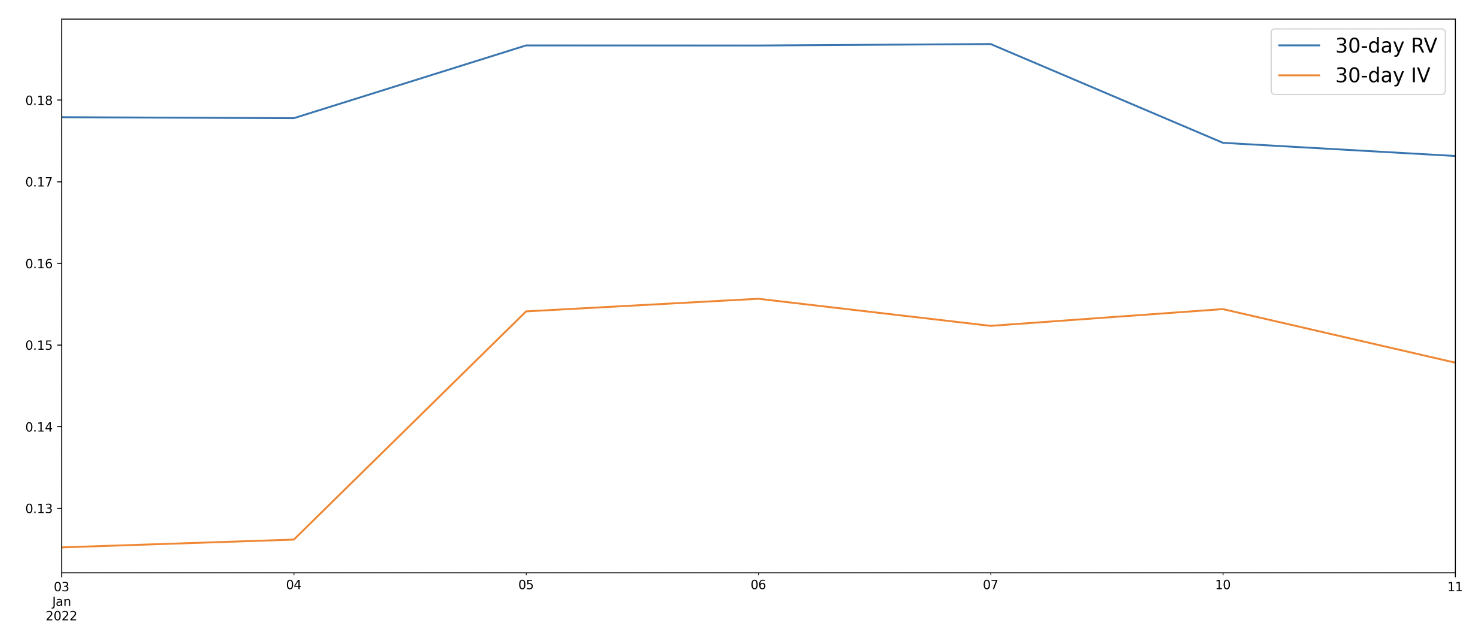
\includegraphics[width=0.49\textwidth]{figures/ivrv2022.png}
    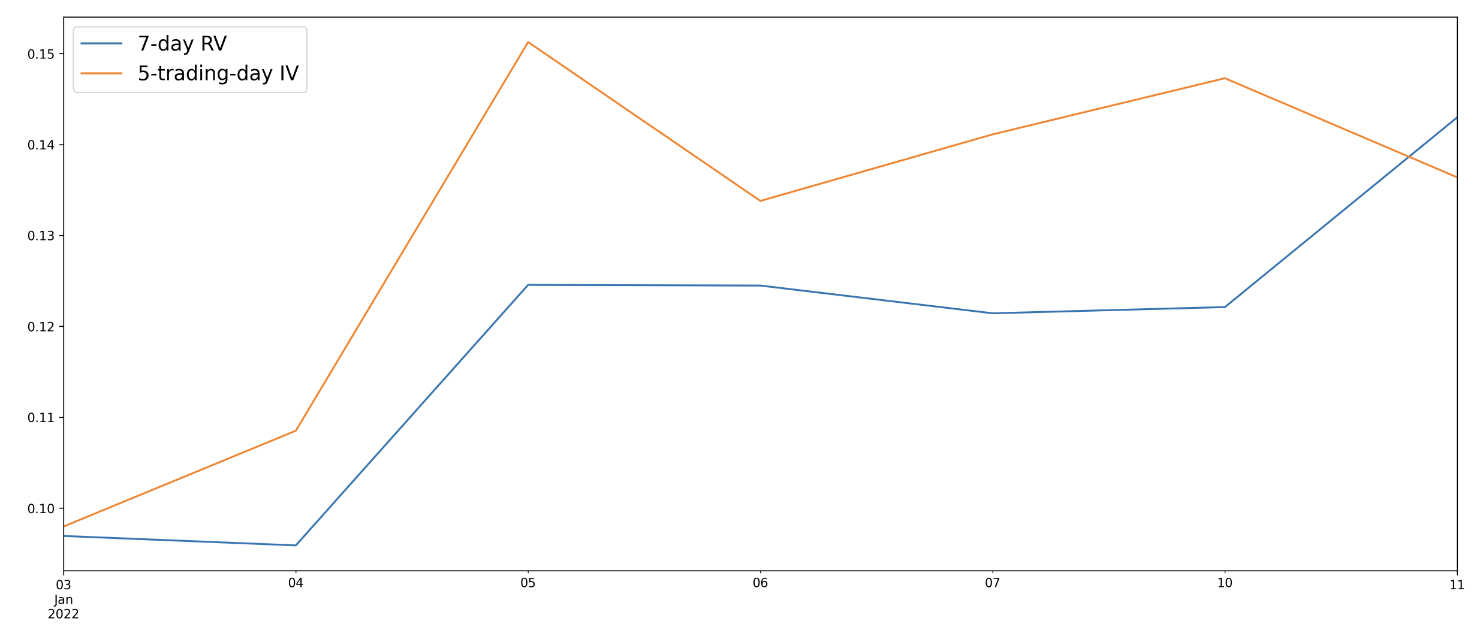
\includegraphics[width=0.49\textwidth]{figures/weekly_ivrv_2022.png}
    \caption{(Left) 30-day Implied vs Realized Volatility During 2022. (Right) Weekly Implied vs Realized Volatility During 2022.}
    \label{fig:ivrv2022}
\end{figure}

\textbf{Using Machine Learning to Augment Trading Decisions.}
The strategy $S_1$ was able to increase the Sharpe ratio of the unaugmented weekly strangle strategy during IS and OS-B, although decreased returns. $S_2$ was able to increase returns and Sharpe ratio compared to $S_1$, as well as achieve the highest return and Sharpe ratio out of all the strategies in our paper for OS-A. It also had the highest Sharpe ratio of 2.59 out of all strategies in the paper for OS-B, but with a very modest 3.77\% return. Furthermore, $S_2$ was able to achieve a Sharpe ratio of > 1 for all its tested periods. Overall, with the exception of success during OS-A, returns are the most modest compared with the other strategies. This suggests that ML was able to trade well but rather conservatively, and that the Random Forest models were indeed able to capture some overfitting information even with overfitting issues.

\section{Conclusion}
In this report, we present a portfolio of strategies that trade on volatility of stock indexes. We demonstrate that our strategies perform well during a variety of in-sample and out-of-sample backtesting periods. We are able to achieve strong positive returns in our portfolio of strategies during all these periods. Furthermore, our strategies achieve very low drawdowns that usually last only a few months; the drawdown values are usually maintained under 10\%, and often even less than 5\% during several periods. 

Our portfolio of strategies present multiple techniques for harvesting different volatility premiums. As demonstrated in our discussion, there may be periods where a certain volatility premium may not exist, or be difficult to capture. During these periods, another strategy can make up for this by capturing a different volatility premium. By combining these strategies, we provide a portfolio that is consistently successful at generating strong positive returns for our investors.

\section*{Acknowledgements}
This report is possible thanks to the support and ideas of Dr. David Ye. In particular, we would like to credit Dr. Ye for the idea on our Skew Arbitrage strategy, who proposed the idea for this approach. We would like to acknowledge the valuable guidance provided by him for our portfolio strategies.

% \printbibliography

% \begin{thebibliography}{99}  
% \bibitem{ref1}Dierckx, T., Davis, J., Schoutens, W. (2022). Trading the FX volatility risk premium with machine learning and alternative data. The Journal of Finance and Data Science, 8, 162–179.
% \bibitem{ref2}Gurdip Bakshi, Nikunj Kapadia, Delta-Hedged Gains and the Negative Market Volatility Risk Premium, The Review of Financial Studies, Volume 16, Issue 2, April 2003, Pages 527–566, 
% \bibitem{ref3}Bhat, A. (2021). The Profitability of Volatility Trading on Exchange-traded Dollar-rupee Options: Evidence of a Volatility Risk Premium? Global Business Review, 0(0). 
 
% \end{thebibliography}

\bibliographystyle{plainnat}
\bibliography{references}

\section*{Supplementary Material}
\subsection*{Future Work}
\subsubsection*{Kelly's Criterion for Optimal Stop-loss Threshold}
Future work for our strategy could involve incorporating Kelly's formula to calculate the best stop-loss threshold. Kelly's criterion tells us that depending on the expected return/loss of the specific trade, each trade has a different theoretically optimal stop-loss threshold. The stop-loss threshold is essentially the variable $a$ in Kelly's criterion. If we have an algorithm that can predict the probability of profit/loss, since the expected profit is known at the beginning of each trade, we could theoretically calculate the expected loss from the formula. Doing so would give us the most optimal capital allocation for each trade. Kelly's formula could prevent a series of inevitable bad trades from wiping out our portfolio in the long term. 

\subsubsection*{Exploring Alternative Underlying Assets}
As was discussed in Section 4.3 on Portfolio Diversification, the correlation among the assets selected (SPY, QQQ, XLF) was too high. Moreover, SPY itself is already a diversified index. Coupled with the fact that drawdowns for our strategies were low due to conservative stop-loss thresholds, diversification failed to improve our results. Future work on this section would be to identify other uncorrelated options and utilize more leverage with such diversified portfolios. One possibility is to explore equity-based options for underlying assets not included in SPY. Another possibility is to explore Forex futures, which are less directly correlated with SPY.

Furthermore, it would be interesting to apply our strategies to other classes of option contracts. There is research on the presence of volatility risk premiums in the foreign exchange markets \citep{BhatRupeeDollar, dierckx_trading_2022} as well as futures options markets, such as the oil market \citep{BouchouevOil}. It would be interesting to explore applications of our strategies in these classes of options as well.

\subsubsection*{Using ML model better suited for time series}
Random forests are not ideal for time series data, as during training, each tree's training subset and test subset can come from the same time period, which is not a valid cross validation split for temporal data. Therefore, the random forest will tend to memorizing time periods or features correlating to time periods rather than features that hold across different time periods. We see that in spite of these issues, Random forests can provide significant alpha extracted from just market data for short term strangle trading. This suggests that a more sophisticated method or even an in depth analysis could yield very good results.

\subsection*{Backtest Figures}
In this section, we share some figures for the returns of our strategies over various testing periods.

\begin{figure}[]
    \centering
    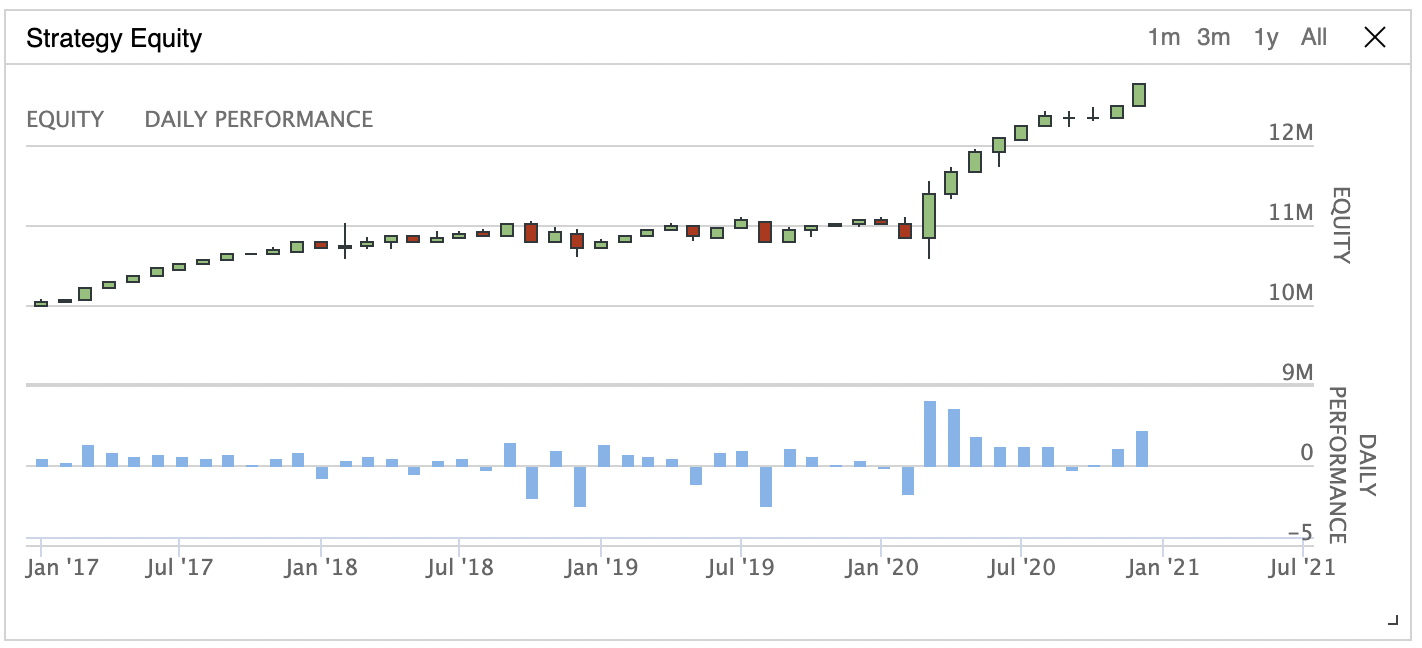
\includegraphics[width=\textwidth]{figures/StraddleInSample.png}
    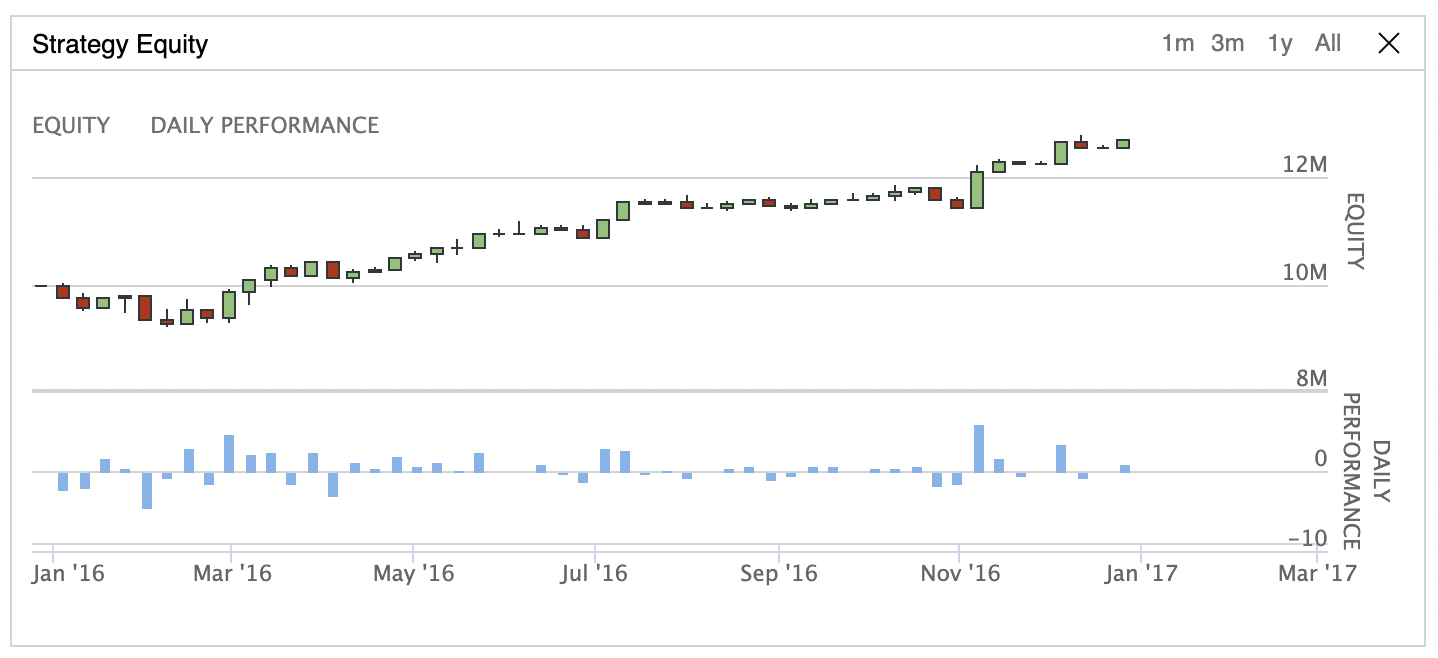
\includegraphics[width=\textwidth]{figures/straddle-2016.png}
    \caption{Returns from the \textbf{Short Straddle Strategy}. (Top) Results from in-sample period 2017-2021. (Bottom) Results from out-of-sample 2016-2017.}
    \label{fig:my_label}
\end{figure}


\begin{figure}
    \centering
    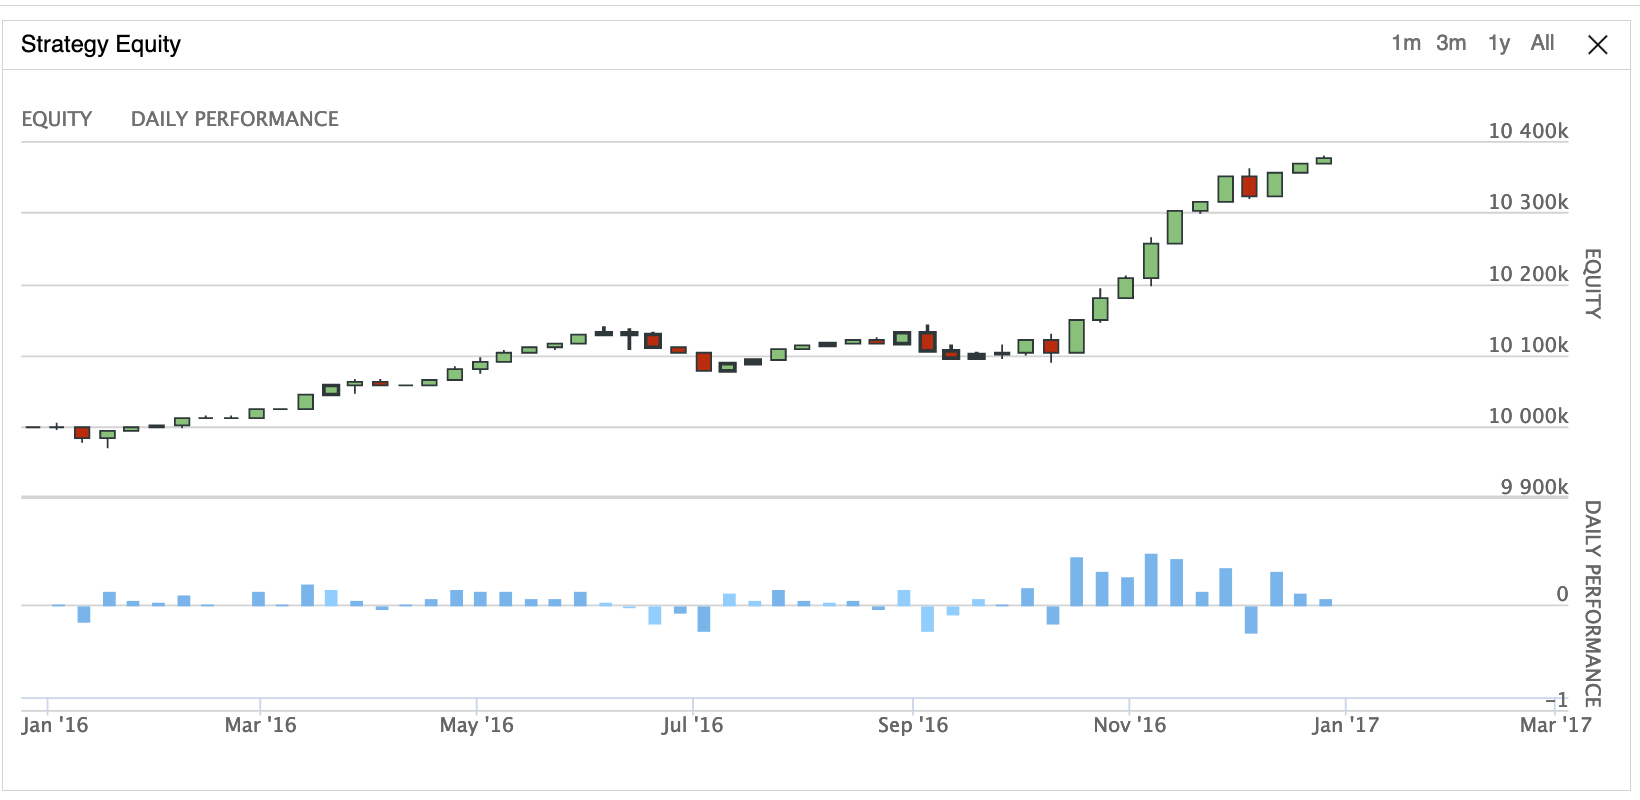
\includegraphics[width=\textwidth]{OSB-RF-S2.png}
    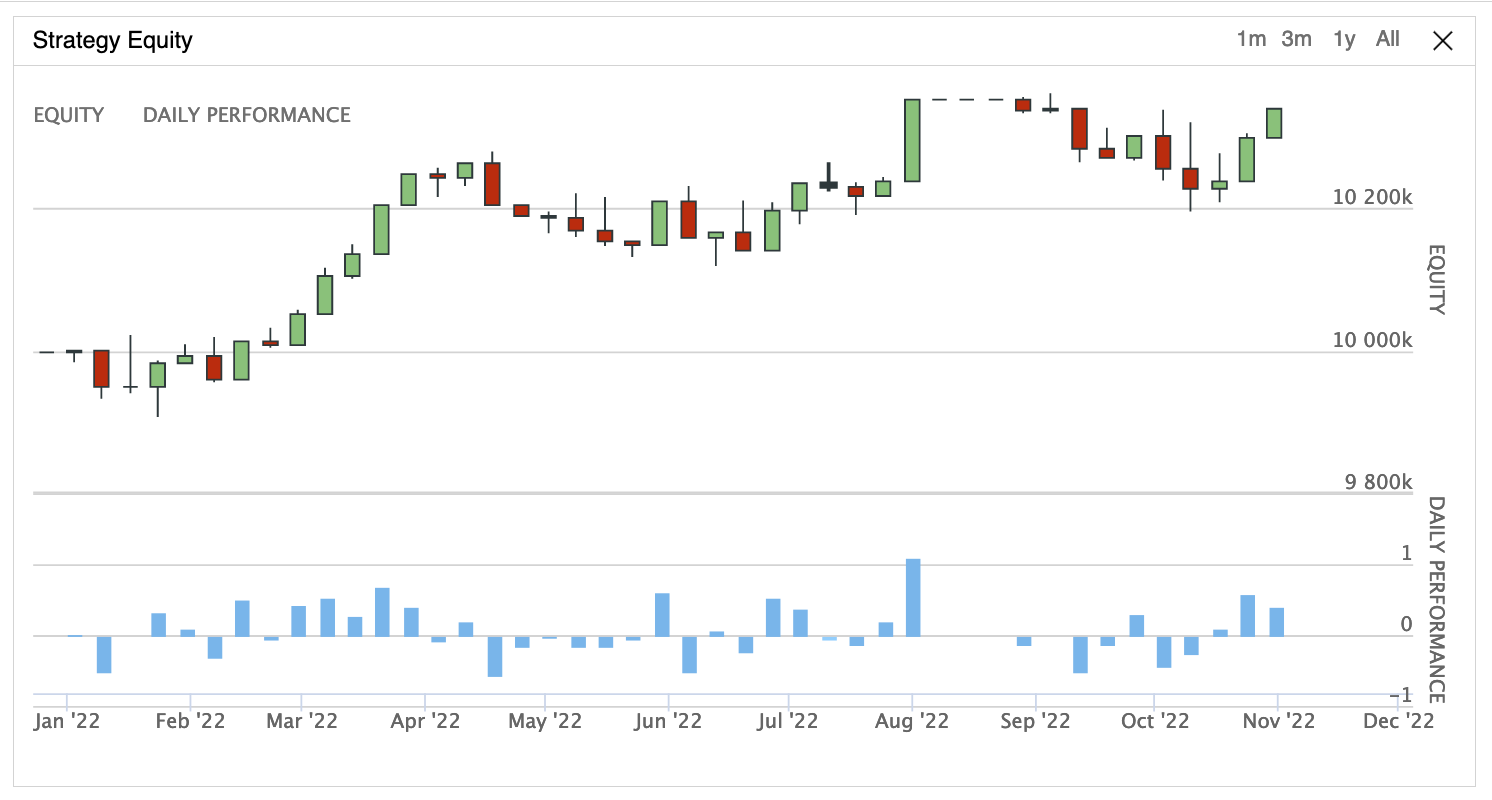
\includegraphics[width=\textwidth]{OSA-RF-S2.png}
    \caption{Returns from the \textbf{Strangle Strategy with Random Forest, $S_2$}. (Top) Results from out-of-sample period 1/1/2016-11/1/2017. (Bottom) Results from out-of-sample period 1/1/2022-11/1/2022.}
    \label{fig:my_label}
\end{figure}

\begin{figure}
    \centering
    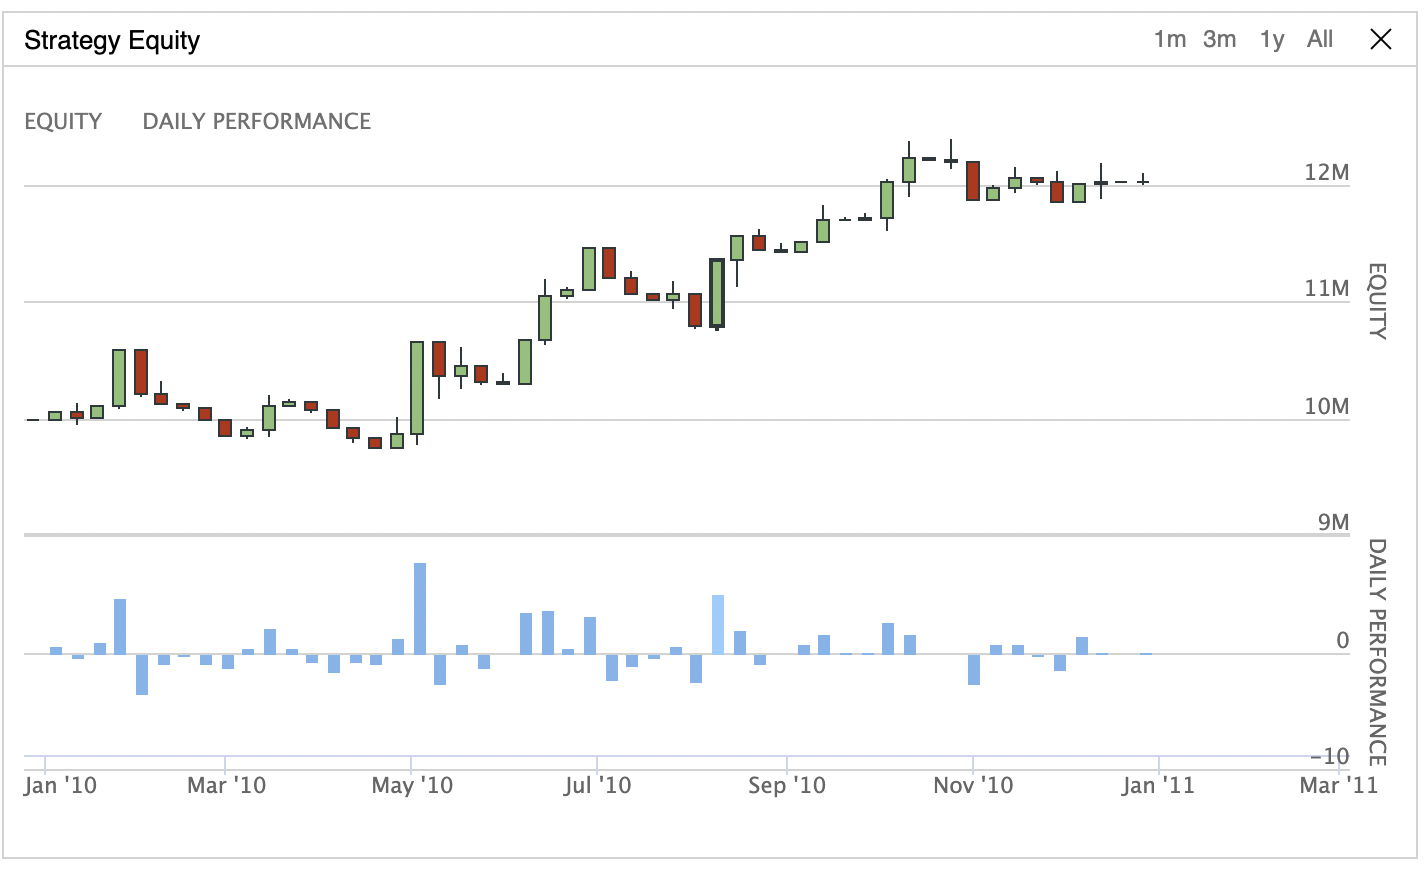
\includegraphics[width=\textwidth]{figures/skew-2010.png}
    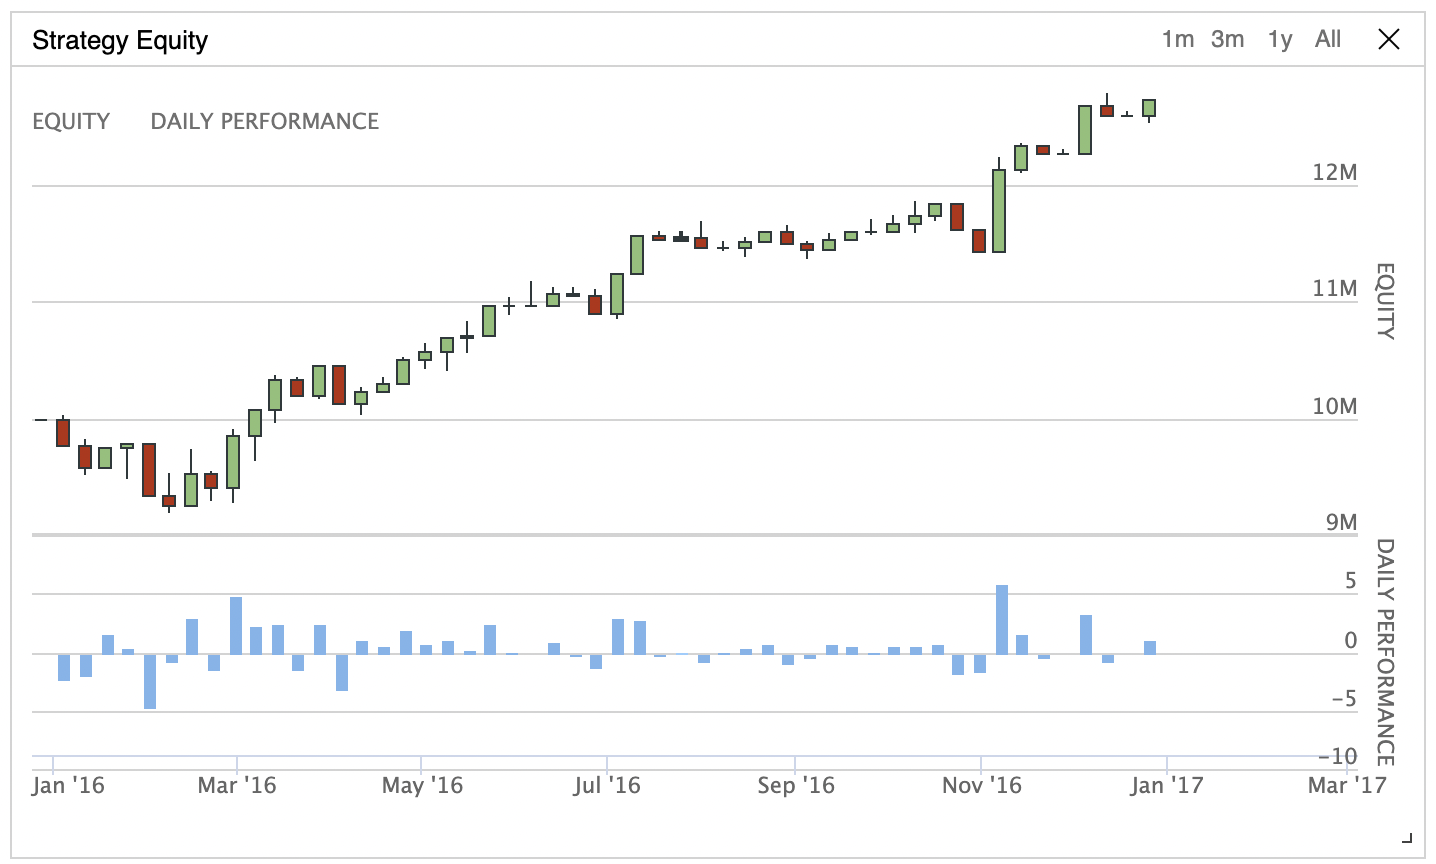
\includegraphics[width=\textwidth]{figures/skew-2016.png}
    \caption{Returns from the \textbf{Skew Arbitrage Strategy}. (Top) Results from 2010-2011. (Bottom) Results from 2016-2017.}
    \label{fig:my_label}
\end{figure}

\begin{figure}[]
    \centering
    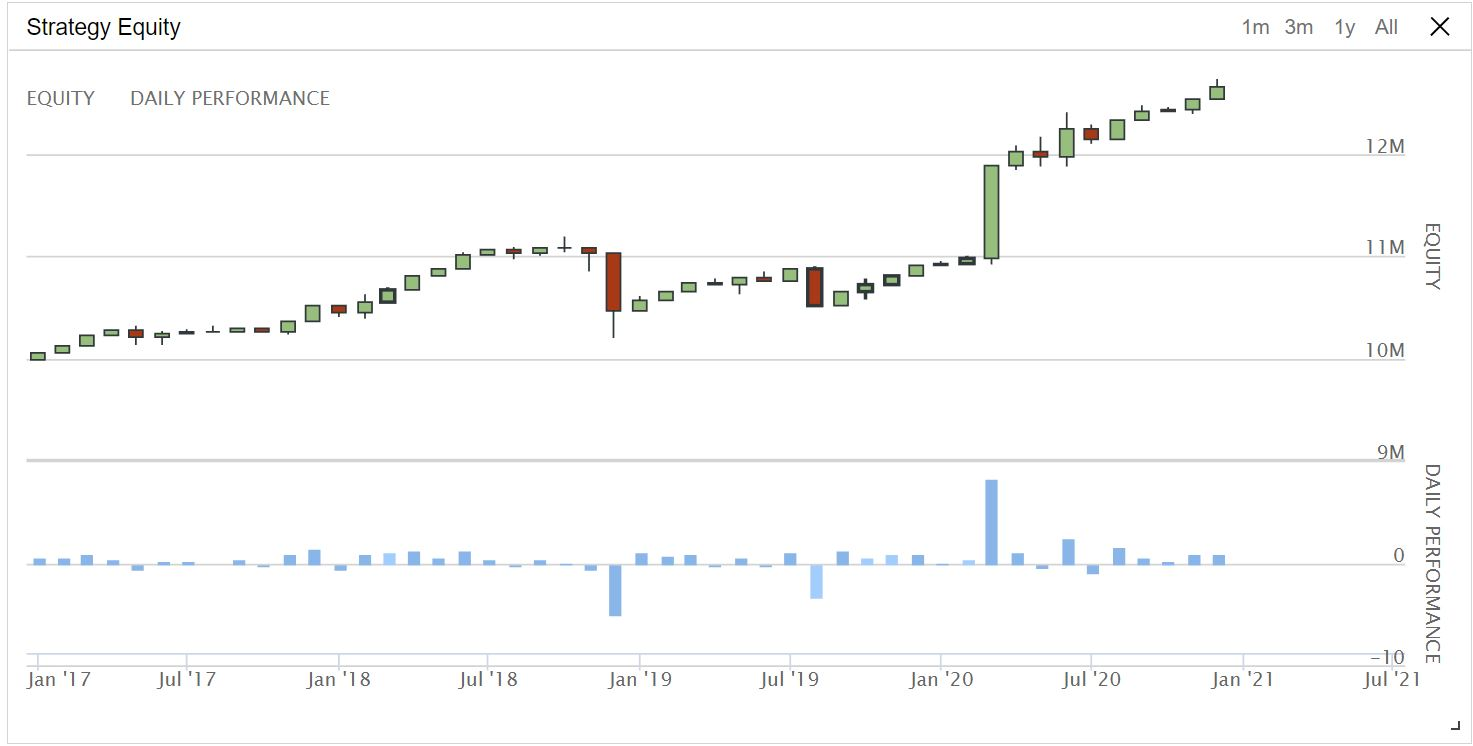
\includegraphics[width=\textwidth]{diverse_xvm_spy_IWM.JPG}
    \caption{SPY, XLV, IWM Returns for In-Sample Period (2017-2021)}
    \label{fig:my_label}
\end{figure}


\end{document}
